%%%%%%%%%%%%%%%%%%%%%%%%%%%%%%% main.tex %%%%%%%%%%%%%%%%%%%%%%%%%%%%%%%
%                                                                      %
% --------------------- Report Template IST [EN] --------------------- %
%                                                                      %
%       João Marafuz Gaspar                                            %
%       Departamento de Engenharia Eletrotécnica e de Computadores     %
%       Instituto Superior Tecnico                                     %
%       Av. Rovisco Pais                                               %
%       1049-001 Lisboa                                                %
%       Portugal                                                       %
%       E-mail: joao.marafuz.gaspar@tecnico.ulisboa.pt                 %
%                                                                      %
%  Created:       Jul 30, 2022                                         %
%  Last Modified: Jul 30, 2022                                         %
%                                                                      %
%%%%%%%%%%%%%%%%%%%%%%%%%%%%%%%%%%%%%%%%%%%%%%%%%%%%%%%%%%%%%%%%%%%%%%%%
%  Revision history                                                    %
%  v1 - 2022/07/30 - original template                                 %
%%%%%%%%%%%%%%%%%%%%%%%%%%%%%%%%%%%%%%%%%%%%%%%%%%%%%%%%%%%%%%%%%%%%%%%%
%                              Preamble                                %
%%%%%%%%%%%%%%%%%%%%%%%%%%%%%%%%%%%%%%%%%%%%%%%%%%%%%%%%%%%%%%%%%%%%%%%%

% ----------------------------------------------------------------------
% Set the document class
% ----------------------------------------------------------------------
\documentclass[12pt,a4paper,oneside]{memoir}

% ----------------------------------------------------------------------
% Define external packages, language, margins, fonts, new commands 
% and colors
% ----------------------------------------------------------------------
\usepackage[utf8]{inputenc} % Codification
\usepackage[english, french]{babel} % Writing idiom

\usepackage{float}

\addto\captionsfrench{\def\tablename{Tableau}}

\usepackage[export]{adjustbox} % Align images
\usepackage{amsmath} % Extra commands for math mode
\usepackage{amssymb} % Mathematical symbols
\usepackage{anysize} % Personalize margins
    \marginsize{2cm}{2cm}{2cm}{2cm} % {left}{right}{above}{below}
\usepackage{appendix} % Appendices
\usepackage{cancel} % Expression cancellation
\usepackage{caption} % Figure numeration
\usepackage{cite} % Citations, like [1 - 3]
\usepackage{color} % Text coloring
\usepackage{fancyhdr} % Head note and footnote
    \pagestyle{fancy}
    \fancyhf{}
    \fancyhead[C]{\footnotesize Analyse et conception d’un module d’apprentissage de la chimie dans un environnement immersif basé sur la réalité virtuelle } % Left of Head note
    \fancyfoot[L]{\footnotesize Rédigé et Présenté par MEVA'A JULES JUNIOR.} % Left of Footnote
    \fancyfoot[R]{\thepage} % Center of Footnote
    \renewcommand{\footrulewidth}{0.4pt} % Footnote rule
\usepackage{float} % Utilization of [H] in figures
\usepackage{graphicx} % Figures in LaTeX
\usepackage[colorlinks = true, plainpages = true, linkcolor = istblue, urlcolor = istblue, citecolor = istblue, anchorcolor = istblue]{hyperref}
\usepackage{indentfirst} % First paragraph
\usepackage{siunitx} % SI units


\providecommand{\keywords}[2]{\textbf{\textit{#1 ---}} #2}
% Random text (not needed)
\usepackage{lipsum}
\usepackage{duckuments}

\usepackage{afterpage}

% Chapter display
\usepackage[T1]{fontenc}
\usepackage{titlesec}

% Array
\usepackage{array,multirow,makecell}
\usepackage{tabularx}
\setcellgapes{1pt}
\makegapedcells
\newcolumntype{R}[1]{>{\raggedleft\arraybackslash }b{#1}}
\newcolumntype{L}[1]{>{\raggedright\arraybackslash }b{#1}}
\newcolumntype{C}[1]{>{\centering\arraybackslash }b{#1}}

% New and re-newcommands
% \newcommand{\sen}{\operatorname{\sen}} % Sine function definition
% \newcommand{\HRule}{\rule{\linewidth}{0.5mm}} % Specific rule definition
% \renewcommand{\appendixpagename}{\LARGE Appendices}


% Colors
\definecolor{istblue}{RGB}{3, 171, 230}
\definecolor{dkgreen}{rgb}{0,0.6,0}
\definecolor{gray}{rgb}{0.5,0.5,0.5}

\setsecnumdepth{subsection}
\setsecnumdepth{subsubsection}
\setsecnumdepth{paragraph}
\setsecnumdepth{subparagraph}

%%%%%%%%%%%%%%%%%%%%%%%%%%%%%%%%%%%%%%%%%%%%%%%%%%%%%%%%%%%%%%%%%%%%%%%%
%                                 Document                             %
%%%%%%%%%%%%%%%%%%%%%%%%%%%%%%%%%%%%%%%%%%%%%%%%%%%%%%%%%%%%%%%%%%%%%%%%
\begin{document}

\chapter*{Dédicace}

{\LARGE À MA FAMILLE}

\chapter*{Remerciements}         % ne pas numéroter
\phantomsection\addcontentsline{toc}{chapter}{Remerciements} % inclure dans TdM

Ce mémoire est l'aboutissement d'une somme d'efforts que nous ne saurions passer sous silence, nous pensons notamment à :

\begin{itemize}
    \item Notre superviseur \textbf{Dr ENGA Vincent} pour sa contribution à l'amélioration de la qualité de ce mémoire,
    \item Notre encadreur académique  \textbf{M. TCHOUTA Alain Serge} pour sa disponibilité et ses conseils pendant le travail,
    \item  Notre encadreur professionnel \textbf{M. KITIO Christian} pour son expertise technique et le suivi au cours du projet,
    \item Au Président Fondateur \textbf{M. GUIMEZAP Paul} pour l’accueil dans son établissement scolaire,
    \item Au Directeur Général de Monglo Technology, \textbf{M. MONGLO Germain} pour sa générosité qui a permis que l'on soit accueilli au sein de son entreprise,
    \item Aux enseignants de l’IUC pour les connaissances apportées et leurs conseils,
    \item Aux amis qui n’ont cessé de m’encourager et de me motiver,
\end{itemize}

\renewcommand\contentsname{Sommaire}
\tableofcontents % Table des matières

\begin{abstract}

    % \keywords{Mot clé}{one, two, three, four}
\end{abstract}
\selectlanguage{english}
\begin{abstract}
	\ac{ict} is constantly evolving and always offers new, simpler and faster ways of carrying out tasks through innovative technology.
    This is the case of virtual reality which allows the simulation of various 3D environments in order to provide users with an immersive experience.
    New applications of this technology in many fields are emerging, especially in education where they allow immersive and safe teaching.
    The objective of this project is to create an immersive chemistry learning environment while limiting the risks associated with its practice for novices.
    Hence the problem of knowing, \pben
    In this context, the facilitation of teaching requires a limitation not only of the costs linked to the teaching of chemistry, but also of the risks linked to its learning by inexperienced people.
    To answer this problem, we have on the one hand identified existing tools allowing a simulated and immersive teaching and on the other hand, we have defined our working methodology thanks to a comparative study between several project management methods (scrum, eXtreme Programming, etc.).
    After this comparative study, our choice fell on Scrum due to the type of project (project with a high risk of change), the project team (very small) and for the iterative aspect it brings to management. of project.
    Then an analysis was carried out on the basis of UML.
    For the implementation in terms of technology, we chose unreal engine 5 for the development of the virtual environment in 3D, react and react dom for the implementation of the web application, PostgreSQL as the database management system and finally Asp.net for the backend implementation.
    From these choices, we have come up with the design of a platform that meets the requested specifications, a web application for managing reactions and a 3D one for practicing these reactions.

	\keywords{Keyword}{Virtual reality, 3D, education, immersion, chemistry, web}
\end{abstract}
\selectlanguage{french}
\chapter*{Introduction}         % ne pas numéroter
\phantomsection\addcontentsline{toc}{chapter}{Introduction} % inclure dans TdM

Avec l'évolution constante des technologies de l'information et de la communication, de nombreux domaines de la vie courante ont changé ou sont en train de changer.
Ces technologies offrent de nouvelle possibilité et permettent une nette évolution dans ces différents secteurs.
Le domaine éducatif bien qu'ancien lui aussi se retrouve touché par cette évolution notamment à cause de la pandémie de la covid-19 qui a touché le monde obligeant son adaptation aux circonstances. 
Ainsi l'enseignement a été délocalisée de nos salles de classe au réseau internet pour un respect des règles de distanciation sociale.
De nouvelles technologies comme la réalité virtuelle ou la réalité augmentée pourraient à leur tour bouleverser le domaine éducatif en introduisant une nouvelle façon d'apprendre (en s'immergeant dans un environnement).
En effet depuis 2012 avec l'arrivée des casques oculus la réalité virtuelle et la réalité augmentée ont subi de grandes évolutions permettant désormais de créer des environnements en trois dimensions à moindre coût et des façons réalistes ces technologies offrent l'avantage d'être virtuel ainsi détaché du monde réel et des risques qui lui sont propres.
Des domaines d'enseignements où ces risques-là sont très présent pourraient bénéficier de cette technologie pour leur enseignement aux novices qui pourraient commettre des erreurs causant des accidents graves voire mortels.
La chimie est l'un des domaines où l'expérimentation dans le monde réel peut avoir de graves conséquences sur l'apprenant ou son environnement du fait de son inexpérience et de la nature des éléments manipulés qui pourraient entrainer des accidents graves.

La réalité virtuelle présente également l'avantage d'être de plus en plus abordable en matière de prix et pourrait permettre aux établissements d'enseignement de faire des économies que ce soit en matière de matériel ou de la main-d'oeuvre.
Dans le cas de la chimie ces économies pourront être faites sur le locale, les équipements, les éléments chimiques et la main-d'oeuvre car tous ces aspects seront simulés.
Dans l'optique d'apporter une solution au problème de savoir \og \pb \fg, nous avons opté pour la réalisation une plateforme et pour ce faire on a pour thème \og \theme \fg.
Le présent document rend compte de tout ce qui a été réalisé durant ce projet. Il s’articule autour de quatre chapitres répartis en deux parties.

La première partie porte sur l’état de l’art, divisée en deux chapitres notamment la présentation du projet et la généralité sur les outils d'apprentissage immersif basé sur la réalité virtuelle.
La deuxième partie intitulée réalisation, comporte deux chapitres, le premier étant l’analyse et la conception, le dernier la réalisation et les résultats.


\part{ÉTAT DE L’ART}
\chapter{PRÉSENTATION DU PROJET}

\textit{Dans ce premier chapitre de la première partie de notre mémoire, nous allons présenter
	notre projet, du contexte à la problématique, sans bien sûr oublier les méthodes. Il présente
	notre projet dans son ensemble, il présente la délimitation du sujet, les problèmes à résoudre,
	l’intérêt du sujet et une étude de l’existant.}

\clearpage

\section{Compréhension du sujet}

\subsection{Contexte}

L’apprentissage est un ensemble de mécanismes menant à l'acquisition de savoir-faire, de savoirs ou de connaissances afin de s’en servir dans la vie courante ou de les faire évoluer pour les générations futures.
Malgré les évolutions technologiques offrant de nouvelles façons d’acquérir des connaissances, le système éducatif africain, plus précisément camerounais n’a pas beaucoup évolué, les moyens de dispenser les connaissances ne suivent pas toujours les tendances actuelles.
Les personnes apprennent mieux en s’immergent dans ce qu’ils font qu’en le théorisant, cela est toujours possible dans le processus d’apprentissage, mais pas dans tous les domaines de formation du fait des risques lié à l’acquisition des connaissances en pratique.

Parmi ces domaines dans lesquels l’immersion réelle des apprenants dans les conditions réelles de pratique présente des risques réels pour l’apprenant, nous pouvons parler de la chimie, qui est un domaine de la science très expérimentale nécessitant des observations pour une compréhension du sujet étudié en vue d’y apporter des applications dans la vie courante.
Une grande et bonne compréhension de ce domaine pourrait apporter de nombreuses idées de recherche qui permettront des avancées significatives dans de nombreux domaines (agriculture, industrie, mode, la mécanique, l'énergie…), avancées qui pourraient à leur tour faciliter le processus d'émergence en Afrique et plus précisément au Cameroun.
Malgré l'aspect très expérimental de son apprentissage, il reste assez dangereux et couteux à enseigner en pratique, dangereux, car le manque d’expérience des apprenants pourrait les pousser à commettre des erreurs qui pourraient causer des accidents très dangereux, voire mortelle en fonction des éléments manipulés et couteux, car la maintenance du matériel nécessaire aux expérimentations (local, verrerie, éléments et personnelles de maintenance) engendre des coûts assez élevés.

\textbf{\ac{vredu}} est une plateforme dont l’objectif est de limiter les coûts et les risques lors des expérimentations en concevant le réalisme afin de créer un sentiment d’immersion pour une meilleure compréhension.
Pour ce faire, monglo technology s’est intéressé à la réalité virtuelle qui est une expression désignant les dispositifs permettant de simuler numériquement un environnement par la machine (ordinateur), afin d’apporter ce réalisme et limiter les risques d’accidents.

\subsection{Délimitation du sujet et hypothèse du travail}

Notre travail se limitera au cas des travaux pratiques de la chimie.

\begin{itemize}
	\item Création des réactions chimiques
	\item Expérimentation des réactions dans un environnement immersif
\end{itemize}

\section{Étude de l’existant}

L’étude de l’existant a pour but d'approfondir l'analyse des axes innovants d'un projet au cours d'élaboration, et avant sa mise en œuvre. Cette étude préalable sert à donner un aperçu sur la pertinence du projet, sa faisabilité ainsi que sa continuité.

\subsection{Description de l’existant}

Nous ne saurions commencer ce travail sans avoir une idée claire et précise sur l’existant quel qu’il soit.
Dans la plupart des lycées, l’enseignement de la chimie suit un modèle traditionnel, à savoir cours théoriques en salle de classe au cours duquel l’apprenant découvre les principes théoriques nécessaires à la maitrise de cette science. Ensuite, un cours pratique en laboratoire au cours duquel les apprenants découvrent la réalité des réactions grâce aux expériences scientifiques.


\subsection{Critique de l’existant et Problématique}

Au cours de notre étude de l’existant, nous avons pu ressortir de nombreux problèmes liés à la réalisation des réactions dans un environnement réel, parmi lesquelles :

\begin{itemize}
	\item Les risques d’accidents au cours d'expérimentation trop élevée dans un environnement réel, accident qui peut s’avérer mortel suivant les éléments manipulés.
	\item Les coûts de maintenance des équipements qui avec le temps se détériorent et nécessitent d’être renouvelé ou entretenu régulièrement ce qui entraine des couts matériels et humains assez importants.
\end{itemize}

Ceci nous a poussé à soulever la problématique : \textbf{\og \pb ? \fg} Autrement dit, pourrait–on envisager une plateforme permettant la simulation d’un laboratoire de chimie en limitant les risques d’accidents au cours des expérimentations et aussi en limitant les coûts de maintenance du matériel une fois l'environnement fonctionnel ?

\subsection{Quelques solutions existantes}

Il est question ici de noter les points forts de ces dernières et leurs points faibles afin d’ajuster nos objectifs.

\begin{itemize}
	\item \textbf{ONTOP DUO MEAC}

	      Ontop duo meac est une technique de simulation de vol utilisé dans les écoles d’aviation utilisé par les formateurs pour mettre en pratique les aspects théoriques abordés durant les formations.
	      En effet, dans le domaine de l’aviation, les simulateurs de vol comme celui-ci sont presque incontournables, car en cas d’accident en condition réel dû au manque d’expérience des apprenants, les nombreuses vies seront menacées et des équipements très coûteux seront détruits.

	      Le dispositif est composé d'écrans disposés à 180° autour de l’apprenant afin de simuler le point de vue d’un pilote et d’un cockpit fidèle à leur homologue réel.

	      \begin{figure}[H]
		      \centering
		      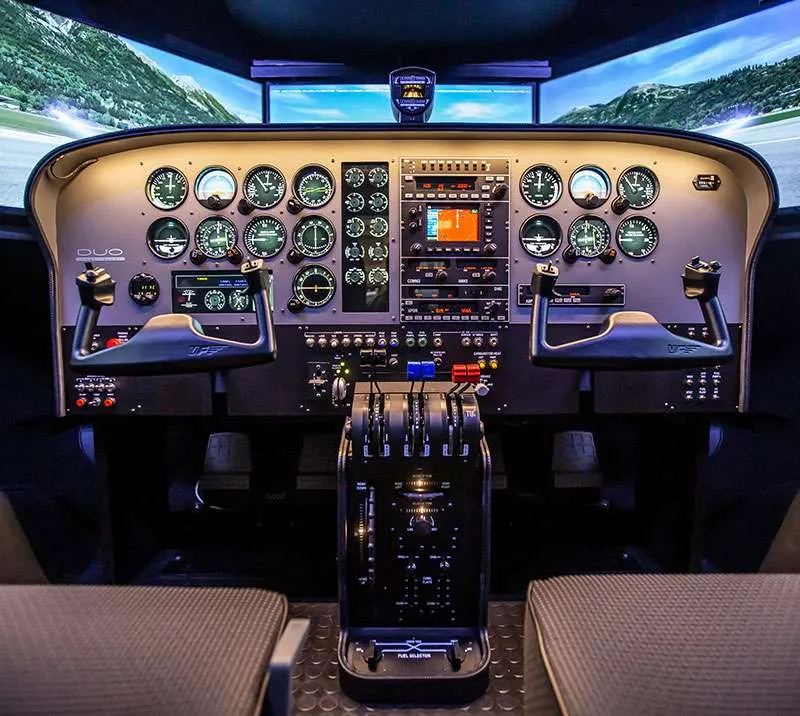
\includegraphics[width=0.5\textwidth]{img/svol1}
		      \caption{Simulateur de vol ONTOP DUO MEAC}
		      \label{fig:mesh1}
	      \end{figure}

	\item \textbf{Microsoft flight simulator}

	      Flight Simulator est un logiciel de simulation de vol pour Microsoft Windows, vendu et souvent vu comme un jeu vidéo. Tout comme l'Ontop duo meac, il permet à l'apprenant de comprendre le domaine de l’aviation en pratiquant à moindre coût car il n’a besoin que d’une console de jeux (PlayStation, Xbox, etc) et de contrôleurs, ici des manettes des consoles ou des dispositifs spéciaux.

	      Cette technique est beaucoup moins rependue dans les centres de formation, car elle est plus adaptée pour les apprenants désireux de s’entrainer chez eux et ne disposant pas des moyens pour un Ontop duo meac.

	      \begin{figure}[H]
		      \centering
		      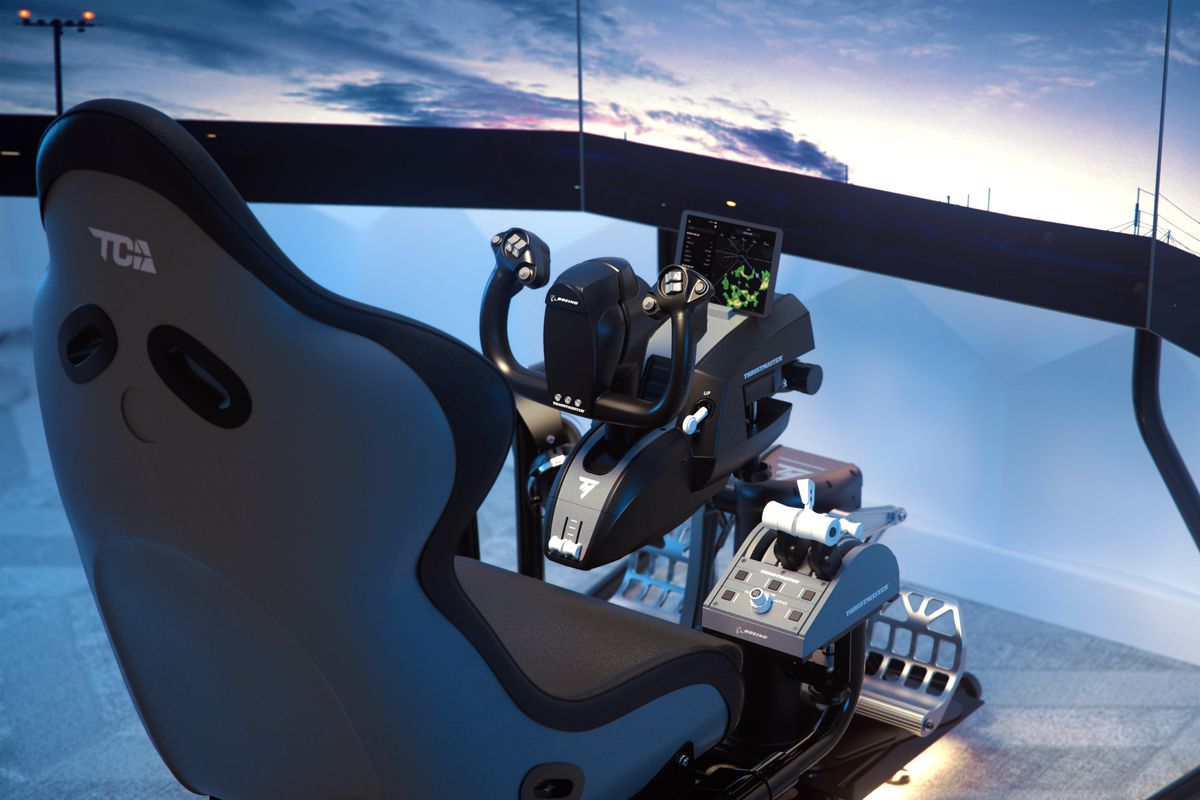
\includegraphics[width=0.5\textwidth]{img/svol2}
		      \caption{Simulateur de vol Microsoft flight simulator}
		      \label{fig:mesh1}
	      \end{figure}

	\item \textbf{Osso VR}

	      Osso VR est une plateforme de formation et d'évaluation chirurgicales qui offre aux entreprises de dispositifs médicaux et aux professionnels de la santé des moyens radicalement meilleurs de partager, de pratiquer.
	      Tout comme dans le domaine de l’aviation, le domaine médical, plus précisément chirurgical utilise des outils de simulation de l’aspect pratique de l’apprentissage.
	      Ceci dû aux risques liés à l’expérimentation sur des individus vivants et le manque de cadavre.

	      Osso VR utilise la réalité virtuelle pour les expérimentations, afin de simuler un monde en trois dimensions représentant un laboratoire dans lequel est disposé un patient virtuel sur lequel seront effectuées les expérimentations.

	      \begin{figure}[H]
		      \centering
		      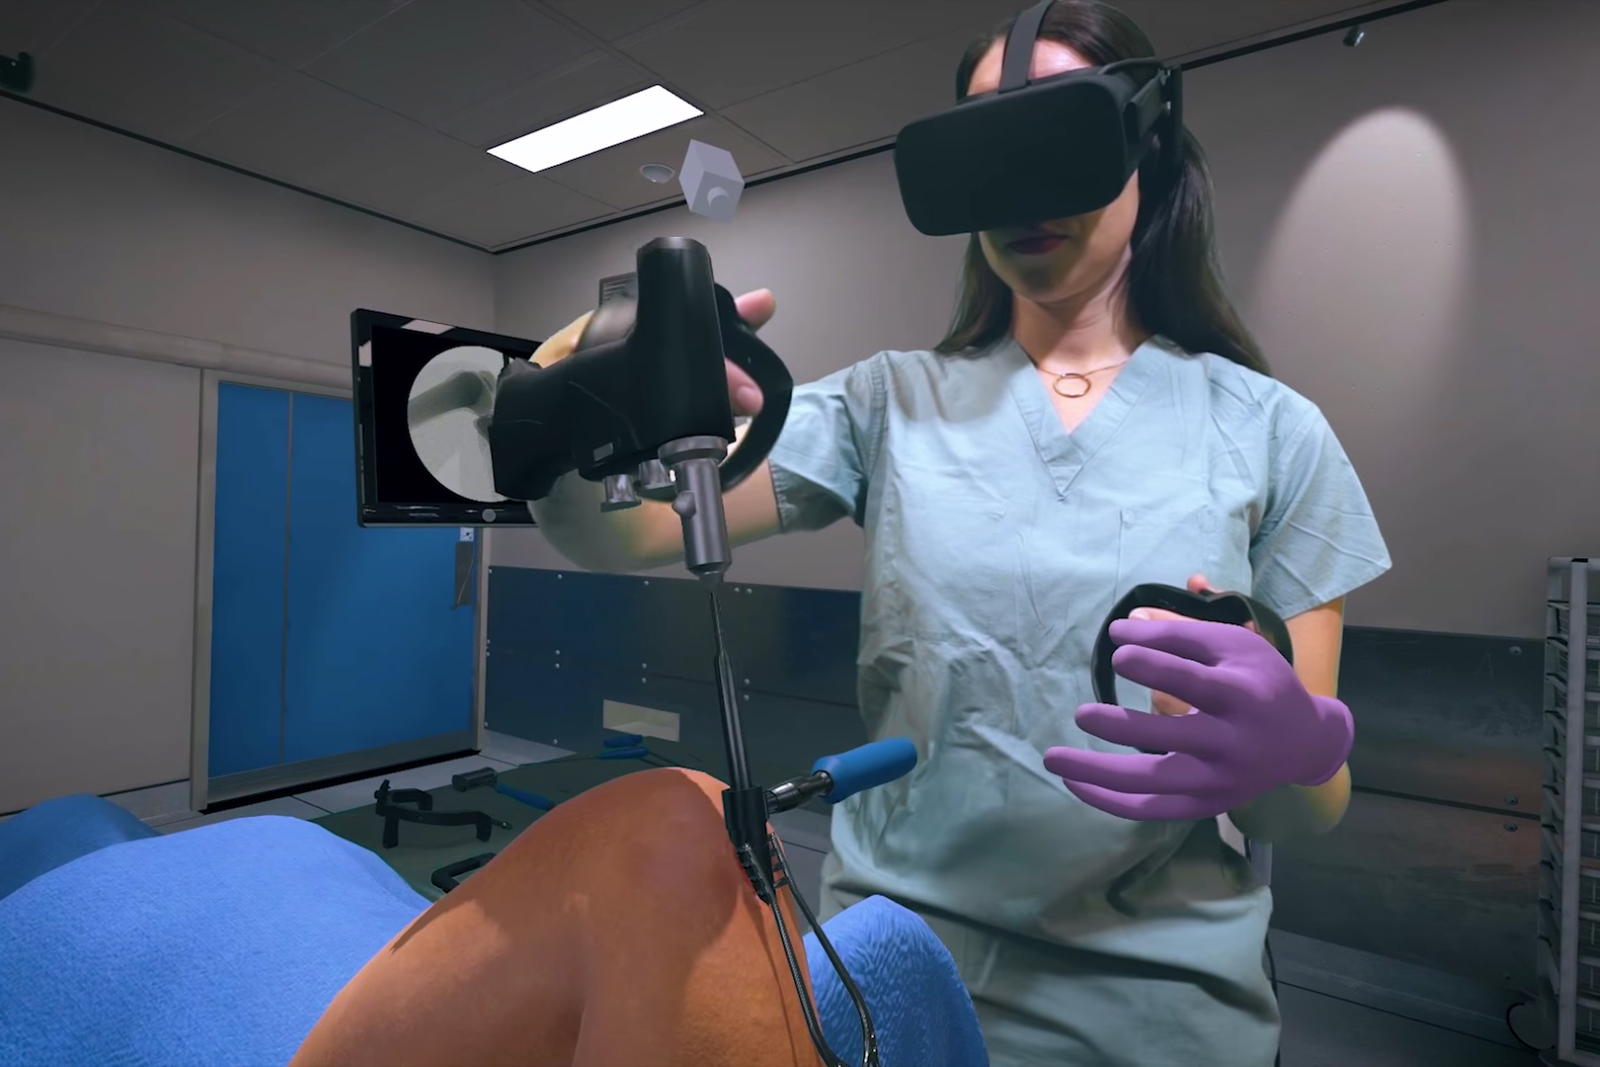
\includegraphics[width=0.5\textwidth]{img/vsurgery}
		      \caption{Simulateur chirurgical Osso VR}
		      \label{fig:mesh1}
	      \end{figure}

	\item \textbf{Praxilab}

	      Praxilab est un outil didacticiel permettant la simulation d'expériences scientifiques dans les domaines de la biologie, la physique et la chimie.
	      Cet outil est développé pour les plateformes desktop et web.
	      Il permet aux apprenants de suivre des instructions afin de réaliser des expériences et comprendre des phénomènes liés aux différents domaines.

	      \begin{figure}[H]
		      \centering
		      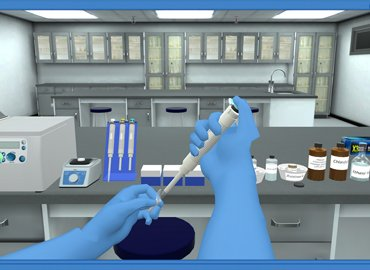
\includegraphics[width=0.5\textwidth]{img/vlab1}
		      \caption{Simulateur scientifique Praxilab}
		      \label{fig:mesh1}
	      \end{figure}

	\item \textbf{EON Reality}

	      EON Reality est une solution de formation académique et industrielle en réalité augmentée et virtuelle.
	      Elle permet l'expérimentation virtuelle dans plusieurs domaines de l’enseignement, à savoir la mécanique, la chimie, la biologie, l’histoire, le génie civil et plein d’autres domaines.

	      Cette solution est disponible sur de nombreux supports à savoir ordinateur sur Windows, casques de réalité virtuelle oculus, sous Android et ios.

	      \begin{figure}[H]
		      \centering
		      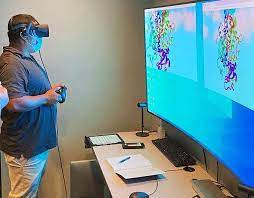
\includegraphics[width=0.5\textwidth]{img/vlab2}
		      \caption{Simulateur scientifique EON Reality}
		      \label{fig:mesh1}
	      \end{figure}
\end{itemize}

\begin{table}[H]
	\centering
	\caption{Comparatif des solutions existantes}
	\begin{tabular}{|l|p{5cm}|p{5cm}|}
		\hline
		\textbf{Application}       & \textbf{Avantages}                                                                                       & \textbf{Inconvénients}                                                         \\ \hline
		ONTOP DUO MEAC             & Très immersif et très réaliste, maintenu et populaire dans le milieu de l'aviation.                      & Trop chère pour une utilisation à domicile, pas adapté aux sciences chimiques. \\ \hline
		Microsoft flight simulator & Assez peu chère à l'obtention donc adapté à une utilisation à domicile et maintenu                       & Pas très immersif et réaliste, pas adapté aux sciences chimiques               \\ \hline
		Osso VR                    & Immersif, assez réaliste et maintenu                                                                     & Disponible seulement en démo, pas adapté aux sciences chimiques.               \\ \hline
		Praxilab                   & Assez réaliste, accessible, adapté aux expérience chimiques et maintenu                                  & Pas très immersif, impossible de créer des réactions, pas de version française \\ \hline
		EON Reality                & Immersif, très polyvalent, disponible sur de nombreuses plateformes et en plusieurs langues, et maintenu & Impossible de créer des réactions                                              \\ \hline
	\end{tabular}
\end{table}

Des outils précédemment présentés, deux ont particulièrement retenu notre attention, car étant beaucoup plus proches de la solution à implémenter. Nous parlons ici de PRAXILAB et EON Reality.

Le tableau ci-dessous fait une présentation plus détaillée de ces deux solutions.

\begin{table}[H]
	\caption{Description des solutions les plus proches de la nôtre}
	\centering
	\begin{tabular}{|l|p{10cm}|}
		\hline
		\textbf{Application} & \textbf{Fonctionnalités}                                                                                                                                                                                                                                                                                                                           \\ \hline
		\textbf{Praxilab}    & Expériences virtuelles immersives en biologie sur des sujets allant de l'extraction d'\ac{adn} et du clonage génétique à la culture tissulaire et à l'électrophorèse des protéines, Expériences virtuelles immersives sur les domaines de la chimie générale, analytique et organique, Expériences virtuelles immersives sur le domaine de la physique. \\ \hline
		\textbf{EON Reality} & Expériences virtuelles, immersives et réaliste des réactions chimiques préenregistrées sur la plateforme                                                                                                                                                                                                                                           \\ \hline
	\end{tabular}
\end{table}



\subsection{Questions de recherche}

\begin{itemize}
	\item Comment pouvons-nous rendre l'enseignement de la chimie moins couteux ?
	\item Comment pouvons-nous rendre l'enseignement de la chimie moins risqué ?
	\item Comment conserver l'aspect réaliste et immersif des expérimentations réelles ?
	\item Comment permettre aux enseignants de créer des réactions pour leurs expérimentations ?
\end{itemize}

\section{Choix et intérêt du sujet}

Le contexte dans lequel nous nous trouvons et la problématique nous oriente vers un
choix de thème qui est \textbf{\og \theme \fg}.
La plateforme \textbf{VREDU Chemistry lab} permettra non seulement de résoudre le problème lié aux coûts de maintenance
du matériel et des infrastructures en limitant aussi les risques au cours des expérimentations.

\section{Objectif du travail}

L’objectif principal est d'apporter un outil d'aide à l'enseignement secondaire, plus précisément de la chimie afin qu'un enseignant puisse créer des réactions que les apprenants suivront durant la phase pratique du cours.

Les objectifs spécifiques sont :

\begin{itemize}
	\item Représentation des réactifs et des produits en trois dimensions et de façon réaliste et immersive
	\item Calcul de la quantité de matière des réactifs dans une solution
	\item Calcul de la concentration des réactifs dans une solution
	\item Calcul de la masse molaire moléculaire des réactifs dans une solution
	\item Calcul du ph d’une solution
\end{itemize}

\section{Méthodologie}

\subsection{Gestion de projet}

Pour le pilotage de notre projet, nous devons choisir parmi les méthodes de gestion de projets une qui convient le mieux non seulement à notre projet, mais également à notre contexte en entreprise.
Pour ce faire, nous allons dans un premier lieu faire une comparaison de ces
méthodes afin de faire un choix convenable.

Alors que les méthodes traditionnelles visent à traiter les différentes phases d’un projet d’une manière séquentielle (que l’on nomme aussi cycle de développement en cascade ou encore cycle
en V), le principe des méthodes Agiles est de le découper en sous-parties (ou sous-projets)
autonomes (on parle également de développement itératif). Les parties (itérations) forment le
projet dans sa globalité.

Nous allons présenter dans un tableau une étude comparative entre l’approche de gestion de projets agiles et celle traditionnelle.


\begin{table}[H]
	\centering
	\caption{Comparaison entre les approches traditionnelles et agiles}
	\label{tab:my-table}
	\begin{tabular}{|l|p{5cm}|p{6cm}|}
		\hline
		\textbf{Thème}      & \textbf{Approche traditionnelle}                                                                       & \textbf{Approche agile}                                                                                                                                              \\ \hline
		Cycle de vie        & En cascade ou en V, sans rétroactions possibles, phases séquentielles                                  & Itératif et incrémental                                                                                                                                              \\ \hline
		Planification       & Produite en quantité importante comme support de communication, de validation et de contractualisation & Réduite au strict nécessaire au profil d’incréments fonctionnels opérationnels pour le feedback du client                                                            \\ \hline
		Équipe              & Contrôle de qualité à la fin du cycle de développement. Le client découvre le produit fini.            & Un contrôle de qualité précoce et permanent au niveau du produit et du processus. Le client visualise les résultats tôt et fréquemment                               \\ \hline
		Qualité             & Une équipe avec des ressources spécialisées et dirigées par un chef de projet.                         & Une équipe responsabilisée ou l’initiative et la communication sont privilégiées et soutenues par le chef de projet                                                  \\ \hline
		Suivi d’avancement  & Mesure de la conformité aux plans initiaux. Analyse des écarts.                                        & Un seul indicateur d’avancement : le nombre de fonctionnalités implémentées et le travail restant à faire.                                                           \\ \hline
		Changement          & Résistance, voire opposition au changement. Processus lourd de gestion des changements acceptés        & Accueil favorable au changement, intègre dans le processus                                                                                                           \\ \hline
		Gestion des risques & Processus distinct, rigoureux de gestion des risques                                                   & Gestion de risques intégrée dans le processus global, avec responsabilisation de chacun dans l’identification et la résolution des risques. Pilotage par les risques \\ \hline
		Mesure du succès    & Respect des engagements initiaux en termes de coût, de budget et ce niveau de qualité                  & Satisfaction client par la livraison de valeur ajoutée                                                                                                               \\ \hline
	\end{tabular}
\end{table}

De cette comparaison, il est possible de choisir, selon le projet, l’approche qui convient le
mieux.

Au vu de notre projet, il convient pour nous de choisir une méthode agile, car cette dernière
s’adapte facilement aux changements et n’impose pas une planification rigide dès le début du
projet. Parmi les méthodes agiles existantes, nous devons en choisir une qui nous convient
encore plus. Après cette comparaison, notre choix s’oriente vers SCRUM.
Car au vu de la grandeur de notre projet, de la taille de l’équipe, des préférences de l’entreprise et de l’approche orientée objet, nous pensons qu’elle est la méthode la mieux adaptée.

\begin{table}[H]
	\centering
	\caption{Comparaison des méthodes agiles}
	\label{tab:my-table}
	\begin{tabular}{|l|l|l|l|}
		\hline
		\textbf{Méthode}                & \textbf{Flexibilité} & \textbf{Itératif} & \textbf{Taille} \\ \hline
		\textbf{Scrum}                  & oui                  & oui               & toute           \\ \hline
		\textbf{Crystal clear}          & oui                  & Non               & petite          \\ \hline
		\textbf{Processus unifié Agile} & oui                  & Non               & toute           \\ \hline
		\textbf{eXtreme Programing}     & oui                  & oui               & petite          \\ \hline
	\end{tabular}
\end{table}

\subsubsection{Qu’est-ce que la méthode SCRUM}

Scrum est un cadre léger qui aide les personnes, les équipes et les organisations à générer de la valeur grâce à
des solutions adaptatives pour des problèmes complexes\cite{schwaber2011scrum}.

Souvent considéré comme un framework de gestion de projets Agiles, Scrum décrit un ensemble de réunions, d'outils et de rôles qui interagissent de concert pour aider les équipes à structurer leur travail et à le gérer.

Scrum est fondé sur l'empirisme et la pensée Lean. L'empirisme affirme que la connaissance vient de l'expérience et de la prise de décisions basées sur ce qui est observé. La pensée Lean réduit le gaspillage et se concentre sur l'essentiel\cite{schwaber2011scrum}.

Scrum utilise une approche itérative et incrémentale pour optimiser la prévisibilité et contrôler les risques. Scrum engage des groupes de personnes qui ont collectivement toutes les compétences et l'expertise pour faire le travail et partager ou acquérir ses compétences selon les besoins. Scrum combine quatre événements formels pour l'inspection et l'adaptation dans un événement conteneur, le sprint. Ces événements fonctionnent parce qu'ils mettent en œuvre les piliers empiriques de Scrum que sont la transparence, l'inspection et l'adaptation.

\vspace{1em}
\begin{itemize}
	\setlength\itemsep{1em}
	\item \textbf{La transparence} : la transparence est un facteur clé de réussite. Tout au long du développement du produit, l’équipe de développement et les parties prenantes ont accès aux informations basées sur un langage et des définitions communs. Par exemple, la définition de fini ou \ac{dod} est obligatoire et très importante pour Scrum. La définition de prêt ou \ac{dor} est aussi une pratique couramment utilisée, mais non obligatoire à ce jour si on se réfère au scrum guide.
	\item \textbf{L'inspection et l'adaptation} : l’équipe doit se consulter quotidiennement pour détecter rapidement d’éventuels écarts entre l’objectif de l’itération (Sprint Goal) et le travail réalisé. Cette Inspection dans le sprint a lieu principalement lors du Daily scrum, de la Sprint Review et de la Sprint Retrospective. Si des écarts sont constatés, un ajustement doit être entrepris afin d’atteindre les objectifs du sprint.

	      L’Inspection et l’adaptation permettent d’ajuster en permanence le développement d’un produit en fonction de l’apprentissage réalisé lors de chaque itération.
\end{itemize}

\subsubsection{Pourquoi la méthode SCRUM}

Cette méthode permet de répondre aux besoins des utilisateurs rapidement, dans les délais
impartis, tout en respectant les budgets. En effet, elle canalise et modélise toutes les étapes du
développement d’un logiciel. Elle ordonne aussi très clairement les différents jalons.

\subsubsection{Avantages de la méthode SCRUM}

Les équipes qui optent pour la structure Scrum gagnent en agilité et en flexibilité. Elle contribue à renforcer la collaboration au sein des équipes et les aide à atteindre leurs objectifs plus efficacement. Par ailleurs, les équipes Scrum savent en permanence sur quoi elles travaillent : elles accomplissent des tâches de leur backlog produit et ont une idée claire de leurs objectifs, car elles se sont concertées sur la définition d’un travail \og terminé\fg.

\subsubsection{Dans quels cas utiliser la méthode SCRUM}

Offrant plus de réactivité, elle est plus adaptée que les méthodes traditionnelles pour la gestion de projets web, tel que le développement logiciel, car elle traduit et organise les projets de façon simple, transparente et pragmatique.

Ce framework, ou cadre de travail, est utile quand :

\vspace{1em}
\begin{itemize}
	\setlength\itemsep{1em}
	\item L’ensemble d’un projet complexe ne peut être ni anticipé ni planifié entièrement.
	\item Son pilotage demande un minimum de flexibilité pour intégrer facilement des changements aux planifications initiales.
\end{itemize}

\subsubsection{Principale contrainte de la méthode SCRUM}

Les projets Scrum souffrent souvent de dérives des objectifs, car cette méthode accepte et encourage le changement. Cependant, il présente des risques d’itérer sans obtenir de résultats concrets si les changements sont trop nombreux ou que les retours clients sont discordants.

\subsection{Analyse et Modélisation}

Pour la réalisation du projet, nous allons procéder comme suit :

\vspace{1em}
\begin{itemize}
	\setlength\itemsep{1em}
	\item Séparation des différents modules à déployer
	\item Développer les différents en utilisant l'approche de développement orienté objet
	\item Déployer ces modules pour la production
\end{itemize}

\subsubsection{L’approche orientée objet}

L’approche orientée objet considère le logiciel comme une collection d’objets dissociés,
identifiés et définis par des propriétés. Une propriété est soit un attribut, soit une méthode.
La fonctionnalité du logiciel émerge alors de l’interaction entre les différents objets qui le
constituent. L’une des particularités de cette approche est qu’elle rapproche les données et
leurs traitements associés au sein d’un unique objet. Un objet est caractérisé par plusieurs
notions dont :

\vspace{1em}
\begin{itemize}
	\setlength\itemsep{1em}
	\item \textbf{L’identité} : l’objet possède une identité, qui permet de le distinguer des autres objets, indépendamment de son état. On construit généralement cette identité grâce à un identifiant
	      découlant naturellement du problème (par exemple une Banque pourra être repéré par un code,
	      un Encaissement par un numéro identifiant, etc.)
	\item \textbf{Les attributs} : il s’agit des données caractérisant l’objet. Ce sont des variables stockant des
	      informations sur l’état de l’objet.
	\item \textbf{Les méthodes} : les méthodes d’un objet caractérisent son comportement, c’est-à-dire l’ensemble
	      des actions (appelées opérations) que l’objet est à même de réaliser. Ces opérations permettent
	      de faire réagir l’objet aux sollicitations extérieures (ou d’agir sur les autres objets). De plus, les
	      méthodes sont étroitement liées aux attributs, car leurs actions peuvent dépendre des valeurs
	      des attributs, ou bien les modifier.
\end{itemize}

La difficulté de cette modélisation réside dans la création d’une représentation abstraite, sous
forme d’objets, d’entités ayant une existence matérielle (Exemple : Banque, Guichet, Caisse, etc.) ou bien virtuelle (Exemple : Encaissement, Décaissement, Transfert de fonds, etc.).
La \ac{coo} est la méthode qui conduit à des architectures logicielles
fondées sur les objets du système, plutôt que sur la fonction qu’il est censé réaliser.

\subsubsection{UML et MERISE}

Les différences entre l’approche objet avec UML et l’approche systémique (fonctionnelle)
avec Merise sont mises en évidence dans l’étude comparative ci- dessous :

\vspace{1em}
\begin{itemize}
	\setlength\itemsep{1em}
	\item \textbf{Points communs} :

	      L’approche classique et l’approche objet distinguent bien globalement trois grandes étapes dans le processus de conception et de développement d’une solution : l’analyse objet correspond au niveau conceptuel de merise, la conception objet est proche de la modélisation logique et organisationnelle de merise.
	      Et enfin l’implémentation objet correspond à la réalisation dans merise.

	      Nous allons reprendre chaque grand niveau de représentation du \ac{si} et donner un certain nombre
	      de précisions sur les points communs.

	      Le niveau de l’analyse objet ou le niveau conceptuel : dans les deux approches, la finalité de ses premiers niveaux de description d’un SI est d’appréhender les besoins à satisfaire et à donner une description de solutions indépendamment des considérations techniques des niveaux logiciels et physiques. Autrement dit, les préoccupations traitées sont très proches malgré des concepts par complètements identiques au niveau conceptuel et au niveau de l’analyse objet.

	      Le niveau conception objet ou le niveau logique organisationnel : ce niveau de description a bien pour finalité dans les deux approches de représenter la solution à implémenter sous l’angle de la logique informatique tant sur la partie des données que sur celle des traitements. Le niveau implémentation physique ou opérationnel dans les deux approches la préoccupation est la description physique et opérationnelle des données et des traitements.

	\item \textbf{Différences} :

	      Nous observons les différences entre ces deux approches au niveau des domaines d’application,
	      de la démarche, les données et les traitements puis l’aspect évolution du système.

	\item \textbf{Les domaines d’application} :

	      Merise a pour vocation de traiter les systèmes d’information des entreprises, principalement dans le domaine de l’informatique de gestion. Le domaine de l’informatique de gestion se caractérise en général par un grand nombre de données à gérer et à stocker avec des traitements relativement peu complexes.

	      Le domaine privilégié par UML est le domaine de l’informatique technique ou industrielle caractérisé par la gestion de composants physiques du monde réel (Informatisation des automates est représentative de ce domaine).
	      Dans ce type de domaine, les aspects traitements d’états et comportements des objets, prennent le pas sur la gestion des données.
	      En plus de cet atout, UML traite également sans difficulté majeure le domaine tel que l’informatique de gestion.

	\item \textbf{La démarche}

	      Avec merise, la démarche est structurée en étapes et phases dont l’étude préalable, l’étude
	      détaillée, la réalisation et la mise en œuvre. Il correspond en effet au cycle de vie d’un système
	      d’information. Et l’ensemble des résultats produits à chaque étape constitue le cycle de décision.
	      Merise propose donc une démarche en cascade, c’est-à-dire qu’une étape ne peut être entamée
	      que si l’étape précédente est achevée. Cela nécessite une organisation minutieuse du projet.
	      Dans le cas contraire, l’on pourrait noter quelques blocages ou une lenteur dans le processus
	      de modélisation du système d’information. Avec UML, la démarche est itérative, incrémentale,
	      guidée par les besoins des utilisateurs du système, et centrée sur l’architecture logicielle. La
	      démarche itérative permet de mieux comprendre et représenter un système complexe. Le
	      périmètre du système à modéliser est défini par les besoins des utilisateurs (les utilisateurs
	      définissent ce que doit être le système).

	\item \textbf{Choix d’une méthode d’analyse}

	      Suite à notre étude comparative entre l’approche systémique avec Merise et l’approche objet avec UML, Nous opterons donc pour une méthode d’analyse suivant l’approche objet dont UML pour la modélisation, dans l’étude conceptuelle de notre système.
	      Ensuite, au vu des circonstances et les délais de notre projet, nous optons pour une démarche itérative, incrémentale, guidée par
	      les besoins des utilisateurs du système. De plus, nous souhaiterions organiser nos programmes
	      en rassemblant les données et les traitements en vue de former des entités cohérentes, logiques
	      et stables. Enfin, nous aimerions faciliter les éventuelles évolutions et maintenances du système.
\end{itemize}

% \subsection{Langages et outils}

% \subsubsection{Choix du langage}


\chapter{GÉNÉRALITÉS SUR LES OUTILS D'APPRENTISSAGE IMMERSIF BASÉ SUR LA RÉALITÉ VIRTUELLE}


\textit{Afin de mener à bien un projet, il est important de comprendre les termes techniques tournant autour du sujet, notre thème porte ainsi sur la réalisation d'un outil d'apprentissage immersif basé sur la réalité virtuelle. Nous allons donc dans ce chapitre expliquer des concepts clés tels que l'apprentissage immersif et la réalité virtuelle}
\clearpage

\section{Apprentissage}

L'apprentissage a été défini fonctionnellement comme des changements de comportement qui résultent de l'expérience ou mécaniquement comme des changements dans l'organisme qui résultent de l'expérience\cite{deHouwer2013WhatIL}.
C'est le processus par lequel les êtres vivants acquièrent et transmettent leurs savoirs.
L'apprentissage a été un sujet central dans la recherche psychologique pratiquement depuis le début de la psychologie
en tant que science indépendante (par exemple, Ebbinghaus, 1885/1962 ; Thorndike, 1911).
Pendant la plus grande partie du siècle précédent, c'était même le sujet le plus étudié en psychologie.
De plus, aujourd'hui, les questions sur l'apprentissage sont abordées dans pratiquement tous les domaines de la psychologie et aussi de l'éducation\cite{deHouwer2013WhatIL}.
De sa définition ressort un principe important, celui de l'expérience, la répétition d'une action qui nous amène à mieux la comprendre.
L'acquisition de cette expérience est le principal défi auquel les organismes éducatifs doivent faire face aux vues du nombre grandissant de techniques et de moyen d'enseignant qui existe, moyens de plus en plus nombreux avec
l'essor des nouvelles technologies telle que le web.

Comme énoncé ci-dessus, il existe un grand nombre de techniques permettant de dispenser ou d'acquérir des connaissances par le moyen de l'apprentissage, parmi lesquelles les plus communément rencontrés sont l'apprentissage traditionnel et l'apprentissage par les jeux.

\subsection{L'apprentissage traditionnel}

Par apprentissage traditionnel, on entend le processus d'apprentissage moderne le plus répandu et le plus ancien qui consiste à dispenser des notions dans un cadre très académique et très strict qui ne laisse donc que peu de liberté d'action ou d'interprétation en limitant toute forme de distraction pour une concentration optimale afin
d'acquérir le maximum de connaissances sur un sujet en un temps données. Bien qu'assez ancienne comme méthode d'enseignement, elle tend à s'adapter à l'époque et aux contraintes auxquelles le monde est soumis notamment par sa digitalisation due aux avancées des \ac{tic} et à la récente pandémie de la covid qui ont créé un bouleversement dans son histoire, si bien que des écoles ou des formations
complètements digitalisées ont vu le jour et offrent des diplômes qui ne présentent aucune distinction de valeur par rapport à ceux obtenus en présentiel. Cela s'explique par le fait que ces deux modes d'études sont considérés comme parfaitement égaux et qu'aucune distinction n'est faite entre eux en matière d'emploi\cite{radovic2010advantages}.

Cette méthode d'apprentissage peut s'avérer très efficace pour l'apprentissage des petits enfants, mais des recherches récentes suggèrent que davantage de méthodes basées sur la découverte pourraient être encore plus efficaces.\cite{Weisberg2018GuidedPlay}

\subsection{L'apprentissage par le jeu}

L'apprentissage par le jeu est une approche pédagogique qui favorise le recours à des activités
ludiques pour stimuler de nombreux aspects du développement et de l'apprentissage de l'enfant\cite{AngelaPyle2018Apprentissage}.
Au début des années 2000, il y a eu un basculement vers la recommandation de l’emploi de
l’apprentissage par le jeu dans les programmes éducatifs préscolaires dans plusieurs pays,
notamment le Canada,\cite{whitebread2009play}
la Suède,\cite{Daubert2018Play}
la Chine,\cite{pyle2017continuum}
les Émirats arabes unis\cite{Hassinger2018Playing}
et la Nouvelle-Zélande\cite{Daubert2018Play}. L'environnement moins académique et moins strict permet aux apprenants de réellement explorer
le sujet soit de manière complètement autonome grâce aux jeux libre\cite{Berk2018Role} dirigé par l'enfant lui-même, soit avec un degré d'encadrement grâce aux jeux dirigés\cite{Bergen2018Cognitive}.

Ce type d'apprentissage est plus ou moins efficace en fonction de l'expérience immersive que propose. En effet, l'opposition des méthodes d'apprentissage par le jeu immersive et non immersive a montré qu'un apprenant aura beaucoup plus de facilité à comprendre un sujet et à s'y intéresser davantage lorsqu'il y est complètement immergé\cite{de2017motivational,Shackelford2019RelationshipsBC,Abdelaziz2020TheIO}.

\subsection{Type d'apprentissage implémenté}

La solution à implémenter sera un outil d'apprentissage combinant ces deux moyens d'apprentissage à savoir, elle se devra non seulement ludique (amusante), mais aussi, l'apprentissage devra être encadré par un enseignant afin que les apprenants suivent le programme défini par l'administration.
\section{La réalité virtuelle et l'éducation}
\subsection{La réalité virtuelle}

Le virtuel peut être défini comme \og étant par essence ou effet, mais pas en fait \fg\cite{Jerald2015WhatIV} et la réalité comme \og l'état ou la qualité d'être réel \fg\cite{Jerald2015WhatIV}.
De la combinaison de ces deux concepts est né un environnement généré par ordinateur avec lequel il est possible d'interagir et de faire l'expérience des sens humains ordinaires comme si l'environnement était réel\cite{Rheingold1991VirtualR}.
La \ac{vr} utilise des combinaisons de matériel informatique et de logiciels pour représenter différents aspects du monde physique à un individu en temps réel.
Un objectif clé de la conception de la réalité virtuelle est d'instiller un sentiment de présence, ou l'illusion d'être immergé dans l'environnement, par opposition à la simple visualisation de l'environnement d'un point de vue extérieur (voir illustration).

\subsubsection{Principe de fonctionnement}

Cinquante ans se sont écoulés depuis que Sutherland a présenté sa vision de l'Ultimate Display\cite{sutherland1965ultimate} imitant le monde réel dans tous les sens disponibles.
Et depuis lors, une grande quantité de technologies individuelles prenant en charge cette stimulation sensorielle ont émergé, mais ce n'est qu'en 1989 que Jaron Lanier a inventé le terme de réalité virtuelle\cite{Rheingold1991VirtualR}.
En 2012, près d'un quart de siècle après la première vague de réalité virtuelle, un projet Kickstarter nommé Oculus Rift, dans le but de fournir au public un écran monté sur la tête abordable et de haute qualité, cherchait un financement et a atteint l'objectif. de 250 000 \$ en moins de 24 heures. Ce fut l'étincelle initiale qui a lancé la deuxième vague de VR\cite{anthes2016state}.
La réalité virtuelle comme tous les domaines des TIC utilisent des périphériques de deux types, à savoir périphériques d'entrée et périphériques de sortie.

Les périphériques d'entrées en réalité virtuelles sont des équipements permettant à l'utilisateur d'interagir avec l'environnement 3D.
Le développement de ces périphériques est très diversifié et remplisse de nombreuses catégories parmi lesquelles nous pouvons citer des casques de réalité virtuelle, des contrôleurs ou manette de réalité virtuelle, des tapis roulant omnidirectionnel, des capteurs de posture, capteur de suivi des gestes\cite{anthes2016state}.

\textbf{Les casques de réalité virtuelle} : est le périphérique de sortie dans l'univers de la réalité virtuel, il permet la visualisation d'environnement 3D grâce à deux écrans disposés comme des lunettes au niveau des yeux de l'utilisateur et de capteur de mouvement permettant à l'utilisation d'un mouvement de tête de changer de point de vue dans l'environnement 3D.
De nombreux équipements l'affiche d'environnement en 3D ont vu le jour ces dernières années parmi lesquelles les plus connus sont : le rift d'oculus, le HTC Vive et le PlayStation VR.

\begin{figure}[H]
	\centering
	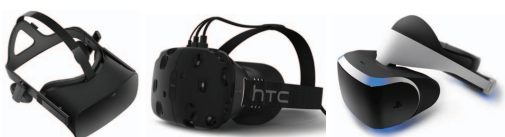
\includegraphics[width=0.5\textwidth]{img/3dcs}
	\caption{L'oculus rift (gauche), le HTC Vive (centre) et le PlayStation VR (droite) }
\end{figure}

\textbf{Les contrôleurs ou manette de réalité virtuelle,} ces équipements sont très proches des manettes traditionnelles utilisées pour des consoles de jeux telles que PlayStation et Xbox mais elles sont plus adaptées à un environnement immersif du fait de leur forme et du positionnement des boutons et des joysticks.
De nombreuses entreprises se sont lancées dans la conception de ces équipements parmi lesquelles nous pouvons citer : l'oculus Half Moon contrôleurs pour des casques de réalité virtuelle de la marque oculus, le steamVR pour le casque HTC Vive et Reactive Grip utilisable sur plusieurs marques de cas de réalité virtuelle parmi lesquelles oculus est vive.

\begin{figure}[H]
	\centering
	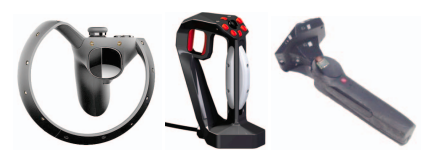
\includegraphics[width=0.5\textwidth]{img/3dcon}
	\caption{L'oculus Half Moon (gauche), le reactive Grip (centre) et le SteamVR (droite) }
\end{figure}

\textbf{Les tapis roulant omnidirectionnel} ce sont des équipements permettant le déplacement dans un environnement 3D en reproduisant les mouvements du monde réel, à savoir la marche, la course et les sauts grâce à un tapis roulant multidirectionnel auquel est attaché le sujet grâce à un harnais afin de suivre et de reproduire ses mouvements.
De nombreux équipements permettant la capture de ses différents mouvements existent parmi lesquelles nous avons : le Space Walker, le walkmouse et l'InfinaDeck.

\begin{figure}[H]
	\centering
	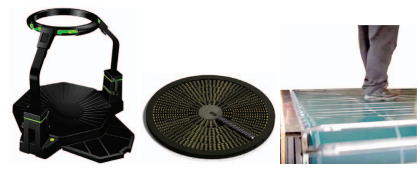
\includegraphics[width=0.5\textwidth]{img/3dtap}
	\caption{Le Virtuix Omni (gauche), le WalkMouse (centre), et le InfinaDeck (droite)}
\end{figure}

\textbf{Les capteurs de posture} ce sont des équipements permettant de reproduire les mouvements du squelette du sujet afin de le reproduire dans l'environnement. Ce type d'équipement créé un sentiment d'immersion dû à une reproduction des mimiques des utilisateurs.
De nombreux équipements permettant la capture de ses différents mouvements existent parmi lesquelles nous avons : le STEM, le PrioVR et ControllVR.

\begin{figure}[H]
	\centering
	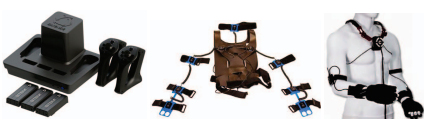
\includegraphics[width=0.5\textwidth]{img/3dcptt}
	\caption{Le STEM (gauche), le PrioVR (centre), et le ControllVR (droite)}
\end{figure}

\textbf{Les capteurs de suivi des gestes} permettant de capturer le mouvement des mains, ils viennent souvent remplacer les contrôler classiques, car moins immersifs et sont souvent utilisés avec le capteur de posture.
De nombreux équipements permettant la capture de ses différents mouvements existent parmi lesquelles nous avons : le Leap Motion, le Myo et le Glove One.

\begin{figure}[H]
	\centering
	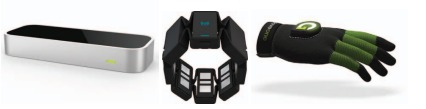
\includegraphics[width=0.5\textwidth]{img/3dgan}
	\caption{Le Leap Motion (gauche), le Myo (centre), et le Glove One (droite)}
\end{figure}

\subsection{La réalité virtuelle et l'éducation}

La réalité virtuelle n'est pas une nouvelle technologie. Mais, plusieurs contraintes ont empêché son adoption effective. Les progrès technologiques récents ajoutés à la prolifération de matériel et de logiciels abordables ont rendu la réalité virtuelle plus viable et souhaitable dans de nombreux domaines, notamment l'éducation; ils ont été relancés avec de nouvelles promesses jusqu'alors inimaginables. La nature de la réalité virtuelle promet de nouveaux modèles d'enseignement et d'apprentissage qui répondent mieux aux besoins de l'apprenant du 21e siècle.
Nous sommes maintenant sur la voie de réinventer l'éducation.

Cette technologie permet désormais d'enseigner en toute sécurité sans risque d'impact réel dans de nombreux domaines d'enseignement telle que la chimie, la biologie, la médecine et bien des domaines ou l'expérimentation est risquée soit pour l'apprenant ou son environnement.

Au cours d'une expérience dans un lycée chinois, lorsque du benzène a été ajouté à un mélange d'acide sulfurique concentré et d'acide nitrique concentré, le mélange s'est soudainement envolé du tube à essai et a éclaboussé les yeux de l'élève impliqué\cite{duan2020mixed}.
Les enseignants et les manuels expliquent très bien les risques liés à ce genre de réaction, mais en raison de leur manque de familiarité avec les procédures expérimentales sûres, les étudiants peuvent oublier les risques pour la sécurité lors de la réalisation d'une expérience\cite{duan2020mixed}.
Ces accidents surviennent également dans les établissements d'enseignement supérieur, comme les universités. Un accident récent s'est produit à l'Université Jiaotong de Pékin qui a causé la mort de trois étudiants qui participaient à l'expérience.
Allant de ce constat Xiaoyun Duan\cite{duan2020mixed} et une équipe de chercheur ont opté pour un dispositif utilisant la réaliter mixte\footnote{La réalité mixte est la fusion de mondes réels et virtuels pour produire de nouveaux environnements et visualisations, où les objets physiques et numériques coexistent et interagissent en temps réel.} pour simuler des réactions afin de créer un environnement sûre pour les apprenants.

Au cours de la dernière décennie, l'application de la technologie VR s'est étendue de l'industrie du divertissement à la médecine clinique. Des chercheurs et des médecins ont exploré les effets de la simulation VR sur la réadaptation physique, la gestion de la douleur, la formation chirurgicale, l'éducation anatomique et le traitement des troubles psychiatriques\cite{li2011virtual, baldominos2015approach, malloy2010effectiveness, alaker2016virtual, yiannakopoulou2015virtual, hackett2016three}.

Le champ d'application de cette technologie ne se limite pas qu'à la chimie et à la médecine, elle peut s'étendre à de nombreux autres domaines, car la seule limite à son utilisation est l'imagination.
\part{RÉALISATION}

\chapter{Cadrage, analyse et conception}

\textit{Comme tout problème qui a été clairement défini, il faut le réaliser mais nous ne pouvons
	parler d’implémentation sans toutefois faire une analyse et une conception. Pour ce faire,
	nous allons cadrer le projet en utilisant la méthode CPS, suivi d’une analyse
	fonctionnelle et non fonctionnelle et bien sûr se terminant par une conception des architectures
	physique et logiques.}

\clearpage

\section{Cadrage du projet}

\subsection{Le projet}

\subsubsection{Le nom}

Le projet à réaliser consiste à pouvoir dispenser les cours (médecine, mathématiques, chimie)
du système éducatif et le travail portera sur le module d’apprentissage de la chimie, d’où le
nom \textbf{vredu chemistry lab}.

\subsubsection{Définition succincte}

\textbf{vredu chemistry lab} sera développée pour la plateforme de réalité virtuelle et les navigateurs web. Elle se devra donc d’être compatible non seulement avec tous les casques de réalité virtuelle de la marque OCULUS mais aussi avec tous les appareils disposant d’un navigateur web. Il sera ainsi possible pour un enseignant de programmer une expérience chimique sur un navigateur web afin que l'apprenant puisse la suivre sur son casque de réalité virtuelle.

\subsubsection{Caractéristiques essentielles}

Notre application sera caractérisée par :

\begin{itemize}
	\item Une Accessibilité sur tous les formats d’équipements numériques de la marque oculus et sur les appareils disposant d’un navigateur web,
	\item Prise en charge des éléments permettant d’effectuer une réaction chimique (éléments du tableau périodique, éprouvettes, béchers, centrifugeuses…).
\end{itemize}

\subsubsection{Motifs qui sous-tendent ce projet}

De nos jours, l’univers numérique offre énormément d'opportunités en ce qui concerne l'acquisition de connaissance grâce à la grande quantité d’information échangée. La chimie est une science dont l'apprentissage se fait de façon expérimentation, expériences entourées de contraintes auxquelles une solution digitale pourrait être la solution à savoir :

\begin{itemize}
	\item Annuler la contrainte du lieu des expérience.
	\item Annuler la contrainte liée à l’acquisition et à la maintenance du matériel d'expérimentation.
	\item Limitation des risques d’accidents. Durant les expérimentations.
	\item Diminution des couts de maintenance et d’acquisition du matériel de laboratoire.
\end{itemize}

\subsection{Les objectifs}

\subsubsection{Objectifs techniques}
\begin{itemize}
	\item \textbf{\underline{Résultats attendus}} : A la fin de ce projet, nous devons avoir deux applications, une pour le web permettant à un enseignant de chimie la création de réaction chimiques auxquelles les apprenants participent par le billet de la seconde application qui elle tournera dans un environnement immersif virtuel.
	\item \textbf{\underline{Objectif principal}} : Obtenir un laboratoire de chimie virtuelle permettant la simulation des réactions chimiques.
	\item \textbf{\underline{Objectifs secondaires}} :
	      \begin{itemize}
		      \item Représentation des réactifs et des produits en trois dimensions et de façon réaliste et immercive
		      \item Calcul des quantités de matière des réactifs dans une solution
		      \item Calcul de la concentration des réactifs dans une solution
		      \item Calcul de la masse molaire moléculaire des réactifs dans une solution
		      \item Calcul du ph d’une solution
	      \end{itemize}
\end{itemize}

\subsubsection{Objectifs de délai}

L’application doit être réalisée dans un délai de sept mois à compter de la date du 10 mai 2022.

\subsubsection{Objectifs de coûts}

\paragraph{Estimation de la main d’œuvre}


\begin{enumerate}
	\item \textbf{Les différents modèles d'estimation des coûts et ressources d’un projet}

	      Au cours de nos recherches, nous avons trouvé de nombreux modèles d’estimation des coûts et ressources d’un projet. Nous pouvons entre autres parlé de :

	      \begin{enumerate}
		      \item \textbf{La méthode descendante} : reste extrêmement populaire dans la gestion de projets contemporains. L'expression « top-down » (descendante) signifie que les instructions sont données en amont. Les objectifs du projet sont fixés par la direction.
		      \item \textbf{La méthode ascendante} : elle se caractérise par une participation proactive de l'équipe dans le processus d'exécution du projet. Les membres de l'équipe sont invités à participer à toutes les étapes du processus de gestion. L'ensemble de l'équipe est amené à décider de la marche à suivre.
		      \item \textbf{La méthode COCOMO} : (acronyme de l'anglais Constructive Cost Model) est un modèle permettant de définir une estimation de l'effort à fournir dans un développement logiciel et la durée que ce dernier prendra en fonction des ressources allouées.
	      \end{enumerate}

	      Sachant que la majeure partie du travail est consacrée à la production du logiciel, nous nous inspirons de la méthode COCOMO pour estimer les coûts de la ressource humaine à ce niveau, lesquels coûts seront inclus dans les coûts globaux de la solution envisagée.

	\item \textbf{Le modèles d'estimation des coûts COCOMO}

	      Cocomo (Constructive Cost Model) est un modèle de régression basé sur le LOC, c’est-à-dire le nombre de lignes de code. Il s’agit d’un modèle procédural d’estimation des coûts pour les projets logiciels et souvent utilisé comme processus de prédiction fiable des divers paramètres associés à la réalisation d’un projet, tels que la taille, l’effort, le coût, le temps et la qualité. Il a été proposé par Barry Boehm en 1970 et repose sur l’étude de 63 projets, ce qui en fait l’un des modèles les mieux documentés. Différents modèles de Cocomo ont été proposés pour prédire l’estimation des coûts à différents niveaux, en fonction de la précision et de l’exactitude requises. Tous ces modèles peuvent être appliqués à une variété de projets, dont les caractéristiques déterminent la valeur de constante à utiliser dans les calculs ultérieurs. Ces caractéristiques propres à différents types de systèmes sont mentionnées ci-dessous :

	      \begin{enumerate}
		      \item \textbf{Organique} – Un projet logiciel est dit de type organique si la taille de l’équipe requise est suffisamment petite, si le problème est bien compris et a été résolu dans le passé et si les membres de l’équipe ont une expérience nominale du problème.
		      \item \textbf{Semi-détaché} – Un projet logiciel est dit de type semi-détaché si les caractéristiques vitales telles que la taille de l’équipe, l’expérience, la connaissance des différents environnements de programmation se situent entre celles de l’organique et de l’Embedded. Les projets classés comme semi-détachés sont comparativement moins familiers et difficiles à développer par rapport aux projets organiques et nécessitent plus d’expérience et une meilleure orientation et créativité. Ex : Les compilateurs ou différents Systèmes Embarqués peuvent être considérés de type Semi-Détachés.
		      \item \textbf{Intégré} – Un projet logiciel nécessitant le plus haut niveau de complexité, de créativité et d’expérience entre dans cette catégorie. Un tel logiciel nécessite une taille d’équipes plus importantes que les deux autres modèles et les développeurs doivent également être suffisamment expérimentés et créatives pour développer des modèles aussi complexes.
	      \end{enumerate}

	      \begin{table}[h!]
		      \caption {types de projet COCOMO}
		      \begin{tabularx}{\textwidth} {
				      | >{\raggedright\arraybackslash}X
				      | >{\centering\arraybackslash}X
				      | >{\raggedleft\arraybackslash}X |}
			      \hline
			      \textbf{Type de projet} & \textbf{Effort en Homme Mois} & \textbf{Temps de Développement} \\
			      \hline
			      ORGANIQUIE              & $2.4(KDSI)^{1.05}$            & $2.5(HM)^{0.38}$                \\
			      \hline
			      MEDIAN                  & $3.0(KDSI)^{1.12}$            & $2.5(HM)^{0.35}$                \\
			      \hline
			      IMBRIQUÉ                & $3.6(KDSI)^{1.20}$            & $2.5(HM)^{0.32}$                \\
			      \hline
		      \end{tabularx}
	      \end{table}

	      Le projet est estimé à 20 KDSI (nombre de milliers d’instructions source livrées) en mode organique (Il est défini par une innovation minimale, une organisation simple en petites équipes expérimentées).

	      % \widowpenalties 3 10000
	      % \raggedbottom
	      \textbf{Formule} :
	      \[E\footnote{E = Effort en Personne-Mois}=2.4\cdot{KLOCx}^{1.05}\]
	      \[D\footnote{D = Durée en Mois.}=2.5\cdot E^{0.38}\]

	      \textbf{Application numérique} :

	      \[E=2.4\cdot10^{1.05}\approx27 Personnes/Mois\]
	      \[D=2.5\cdot 56^{0.38}\approx8 Mois\]

	      \begin{table}[h!]
		      \caption {Estimation des coûts}
		      \begin{tabularx}{\textwidth} {
				      | >{\raggedright\arraybackslash}X
				      | >{\centering\arraybackslash}X
				      | >{\centering\arraybackslash}X
				      | >{\centering\arraybackslash}X
				      | >{\raggedleft\arraybackslash}X |}
			      \hline
			      \textbf{Participant}                    & \textbf{Quantité} & \textbf{Durée en semaine} & \textbf{Cout/Semaine} & \textbf{Cout total} \\
			      \hline
			      \textbf{Chef de projet}                 & 1                 & 4                         & 200.000 XAF           & 800.000 XAF         \\
			      \hline
			      \textbf{Développeur}                    & 1                 & 32                        & 100.000 XAF           & 3.200.000 XAF       \\
			      \hline
			      \textbf{Testeur}                        & 2                 & 1                         & 50.000 XAF            & 50.000 XAF          \\
			      \hline
			      \multicolumn{4}{| l |}{\textbf{Total} } & 4.050.000 XAF                                                                               \\
			      \hline
		      \end{tabularx}
	      \end{table}
\end{enumerate}

\paragraph{Estimation matérielle et logiciel}\mbox{}\\

Ce tableau présente une estimation du matériel selon le besoin et la durée.

\begin{table}[H]
	\caption{Estimation des coûts matériels}

	\begin{tabular}{ |p{7cm}|p{2cm}|p{3cm}|p{3cm}| }
		\hline
		\textbf{Ressource}                                                                                                                                                                                                                                     & \textbf{Nombre de payement} & \textbf{Cout par payement}                   & \textbf{Total} \\
		\hline
		Desktop monté avec les caractéristiques : 32Go de RAM, Une carte graphique Nvidia GeForce GTX 1070, 250Go de disque dur SSD, 1To de disque dur HDD, Processeur Intel core i7 3.60GHz, Boitier et carte graphique predator, Ecran 32 pouces, Clavier HP & 7                           & 23.472 XAF (\textit{Amortissement par mois}) & 164.304 XAF    \\
		\hline
		1 serveur de développement : 100 Go SSD, 4 Go Ram, Ubuntu 20                                                                                                                                                                                           & 7                           & 80.000 XAF                                   & 560.000 XAF    \\
		\hline
		1 serveur git: 2Go RAM, 30 Go HDD, Ubuntu 20                                                                                                                                                                                                           & 7                           & 80.000 XAF                                   & 560.000 XAF    \\
		\hline
		1 casque oculus                                                                                                                                                                                                                                        & 7                           & 5.940 XAF (\textit{Amortissement par mois})  & 41.580 XAF     \\
		\hline
		Connexion Internet haut débit                                                                                                                                                                                                                          & 7                           & 30.000 XAF                                   & 210.000 XAF    \\
		\hline
		Rider                                                                                                                                                                                                                                                  & 1                           & 91.809 XAF                                   & 91.809 XAF     \\
		\hline
		Unreal engine                                                                                                                                                                                                                                          & 7                           & Gratuit                                      & Gratuit        \\
		\hline
		Webstorm                                                                                                                                                                                                                                               & 1                           & 91.809 XAF                                   & 91.809 XAF     \\
		\hline
		\multicolumn{3}{| l |}{\textbf{Total} }                                                                                                                                                                                                                & 1.719.502 XAF                                                                               \\
		\hline
	\end{tabular}
\end{table}

Le coût du matériel est ainsi estimé à : \textbf{1.719.502 XAF}

Ainsi le coût total du projet est de \textbf{5.769.502 XAF }

\subsection{La technique}

\subsubsection{La base sur laquelle le projet s’appuie}

Nous avons déjà eu à réaliser des projets en informatique et en particulier des applications Web, bien que les applications de réalités virtuelles soient pour nous une nouvelle expérience, nous pensons pouvoir y parvenir grâce la communauté qui est nombreuse et également l’aide des professionnels en stage notamment notre encadreur. De plus, les supports de cours, les enseignants et l’internet (possibilité de documentation) sont des atouts majeurs renforçant cet engagement. Des didacticiels dans des environnement 3D existent déjà, ce qui nous fait encore croire encore plus à la réalisation de ce projet.

\subsubsection{Les difficultés principales de ce projet}

\begin{itemize}
	\item Apporter du réalisme aux réactions chimiques
	\item Sécurité de l’application
\end{itemize}

\subsubsection{Les solutions de repli en cas de problème }

Pour le problème lié au réalisme à apporter aux expériences, nous avons pensé à confier la réalisation des assets 3D à des tiers qui nous rémunèrent.

En ce qui concerne la sécurité de l’application, vu que l’application sera hébergée en ligne nous nous informerons sur les différents risques liés à un tel hébergement et tenterons de les éviter lors de la phase de développement.

\subsection{Le planning}

\subsubsection{Dates clés}

\begin{itemize}
	\item Date de début : 10 mai 2022
	\item Date de fin :  03 décembre 2022
\end{itemize}

\subsubsection{Grandes phases du planning}

Pour la gestion du temps, il existe des méthodes de planification prévisionnelle de projet tel que le diagramme de Gantt. Ce dit diagramme regroupe toutes les tâches, les durées et les ressources ordonnées de manière graduelle permettant à toute l’équipe de suivre son évolution. Il peut être modifié au fur et à mesure en fonction des délais respectés ou pas ainsi que des imprévus. Dans le cadre de notre projet, la planification de nos tâches nous a permis de ressortir le diagramme de Gantt suivant :


\begin{table}[H]
	\caption{Estimation des coûts matériels}
	\resizebox{\textwidth}{!}{%
		\begin{tabular}{|lll|l|ll|}
			\hline
			\multicolumn{1}{|l|}{\textbf{Phase}}                            & \multicolumn{2}{l|}{\textbf{Taches}}                                    & \textbf{\begin{tabular}[c]{@{}l@{}}Durée\\  en jour\end{tabular}}                  & \multicolumn{1}{l|}{\textbf{Durée en heure}} & \textbf{Prédécesseurs}         \\ \hline
			\multicolumn{1}{|l|}{\multirow{4}{*}{\textbf{Analyse}}}         & \multicolumn{2}{l|}{Cadrage du projet (A)}                              & 4                                                    & \multicolumn{1}{l|}{36}                      &                                \\ \cline{2-6}
			\multicolumn{1}{|l|}{}                                          & \multicolumn{2}{l|}{Etude l’existant (B)}                               & 5                                                    & \multicolumn{1}{l|}{45}                      & A                              \\ \cline{2-6}
			\multicolumn{1}{|l|}{}                                          & \multicolumn{2}{l|}{Elaboration du diagramme des cas d’utilisation (C)} & 3                                                    & \multicolumn{1}{l|}{27}                      & B                              \\ \cline{2-6}
			\multicolumn{1}{|l|}{}                                          & \multicolumn{2}{l|}{Elaboration des diagrammes de séquence (D)}         & 3                                                    & \multicolumn{1}{l|}{27}                      & B                              \\ \hline
			\multicolumn{1}{|l|}{\multirow{2}{*}{\textbf{Conception}}}      & \multicolumn{2}{l|}{Elaboration du diagramme de classe (E)}             & 5                                                    & \multicolumn{1}{l|}{45}                      & D,C                            \\ \cline{2-6}
			\multicolumn{1}{|l|}{}                                          & \multicolumn{2}{l|}{Elaboration du diagramme de déploiement (F)}        & 1                                                    & \multicolumn{1}{l|}{9}                       & D,C                            \\ \hline
			\multicolumn{1}{|l|}{\multirow{11}{*}{\textbf{Implémentation}}} & \multicolumn{1}{l|}{\multirow{4}{*}{Back end}}                          & Module de gestion des utilisateurs (G)               & 15                                           & \multicolumn{1}{l|}{135} & F   \\ \cline{3-6}
			\multicolumn{1}{|l|}{}                                          & \multicolumn{1}{l|}{}                                                   & Module de gestion des éléments chimiques (H)         & 12                                           & \multicolumn{1}{l|}{108} & G,E \\ \cline{3-6}
			\multicolumn{1}{|l|}{}                                          & \multicolumn{1}{l|}{}                                                   & Module de gestion des équipements de laboratoire (I) & 15                                           & \multicolumn{1}{l|}{135} & H   \\ \cline{3-6}
			\multicolumn{1}{|l|}{}                                          & \multicolumn{1}{l|}{}                                                   & Tests (J)                                            & 2                                            & \multicolumn{1}{l|}{18}  & I   \\ \cline{2-6}
			\multicolumn{1}{|l|}{}                                          & \multicolumn{1}{l|}{\multirow{4}{*}{Front end}}                         & Module de gestion des utilisateurs (K)               & 15                                           & \multicolumn{1}{l|}{135} & J   \\ \cline{3-6}
			\multicolumn{1}{|l|}{}                                          & \multicolumn{1}{l|}{}                                                   & Module de gestion des éléments chimiques (L)         & 15                                           & \multicolumn{1}{l|}{135} & K   \\ \cline{3-6}
			\multicolumn{1}{|l|}{}                                          & \multicolumn{1}{l|}{}                                                   & Module de gestion des équipements de laboratoire (M) & 10                                           & \multicolumn{1}{l|}{90}  & L   \\ \cline{3-6}
			\multicolumn{1}{|l|}{}                                          & \multicolumn{1}{l|}{}                                                   & Tests (N)                                            & 2                                            & \multicolumn{1}{l|}{18}  & M   \\ \cline{2-6}
			\multicolumn{1}{|l|}{}                                          & \multicolumn{1}{l|}{\multirow{3}{*}{Interfaces 3D}}                     & Menus et interface d’accueil (O)                     & 10                                           & \multicolumn{1}{l|}{90}  & N   \\ \cline{3-6}
			\multicolumn{1}{|l|}{}                                          & \multicolumn{1}{l|}{}                                                   & Gestion des réactions chimiques (P)                  & 25                                           & \multicolumn{1}{l|}{225} & N   \\ \cline{3-6}
			\multicolumn{1}{|l|}{}                                          & \multicolumn{1}{l|}{}                                                   & Tests (Q)                                            & 5                                            & \multicolumn{1}{l|}{45}  & O,P \\ \hline
			\multicolumn{1}{|l|}{\textbf{Transition}}                       & \multicolumn{2}{l|}{Tests (R)}                                          & 5                                                    & \multicolumn{1}{l|}{45}                      & Q                              \\ \hline
			\multicolumn{3}{|l|}{\textbf{Total}}                            & \textbf{152}                                                            & \multicolumn{2}{l|}{\textbf{1368}}                                                                                                   \\ \hline
		\end{tabular}%
	}
\end{table}

Ce tableau nous permettra de réaliser notre diagramme Gantt.

\subsubsection{Diagramme Gantt}

Ce diagramme présente le planning général du projet, fait en utilisant le logiciel Gantt Project.

\begin{figure}[H]
	\centering
	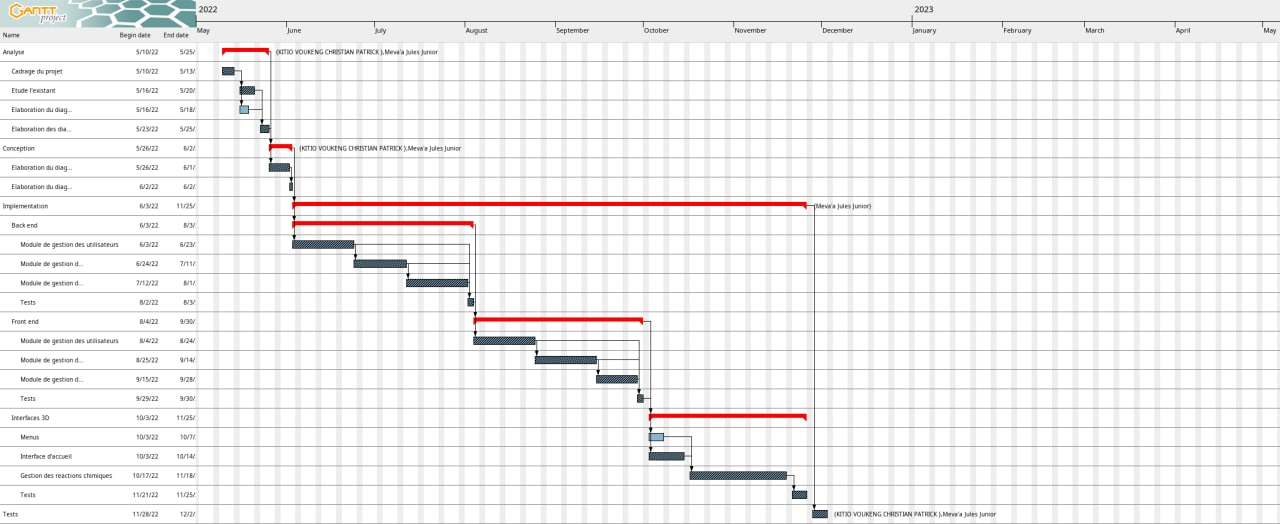
\includegraphics[width=1.3\textwidth, angle=-90]{img/gantt}
	\caption{Diagramme de gantt du projet}
	\label{fig:mesh1}
\end{figure}

De ce diagramme, ressort la date de début du projet qui est le 10 mai 2022 et la date de fin le 03 Décembre 2022. La durée du projet est de 156 jours. Le chemin critique est noté en bleu sombre sur ce diagramme.

\subsection{Les moyens}

\subsubsection{Moyens humains}

Ici nous retrouvons l'équipe chargée de la réalisation du module \textbf{Mr. KITIO VOUKENG Christian PATRICK} directeur technique a monglo-technologie et \textbf{MEVA’A JULES JUNIOR} stagiaire en développement et en management des solutions digitales et datas a monglo-technologie.

\subsubsection{Moyens matériels}

\begin{table}[H]
	\centering
	\caption{Moyens matériels}
	\label{tab:my-table}
	\begin{tabular}{|l|p{7cm}|}
		\hline
		\multicolumn{1}{|l|}{Ordinateurs desktop} & 32Go de RAM, Une carte graphique Nvidia GeForce GTX 1070, 250Go de disque dur SSD, 1To de disque dur HDD, Processeur Intel core i7 3.60GHz, Boitier et carte graphique predator, Ecran 32 pouces, Clavier HP \\ \hline
		\multicolumn{2}{|l|}{\begin{tabular}[c]{@{}l@{}}1 Casque de réalité virtuelle Oculus \\ Quest\end{tabular}}                                                                                                                                                                                                         \\ \hline
		\multicolumn{2}{|l|}{1 serveur git}                                                                                                                                                                                                                      \\ \hline
		\multicolumn{2}{|l|}{1 serveur git}                                                                                                                                                                                                                      \\ \hline
	\end{tabular}
\end{table}

\subsection{Le management du projet}

Pour la réalisation de ce projet, nous disposons des ressources humaines suivantes :

\begin{table}[H]
	\centering
	\caption{Le management du projet}
	\label{tab:my-table}
	\resizebox{\textwidth}{!}{%
		\begin{tabular}{|l|l|}
			\hline
			\textbf{Noms}                       & \textbf{Fonctions}                         \\ \hline
			Mr. KITIO VOUKENG CHRISTIAN PATRICK & Responsable du projet, analyste et testeur \\ \hline
			MEVA’A JULES JUNIOR                 & Analyste, développeur et testeur           \\ \hline
		\end{tabular}%
	}
\end{table}

\subsection{La communication}


\subsubsection{Communication interne du projet}

\begin{itemize}
	\item Collaboration via GitLab
	\item Communication via telegram
	\item Réunion en présentielle ou en ligne (en fonction du contexte) pour l’évaluation de l’évolution du projet et les tests
\end{itemize}

\subsubsection{Communication externe}

\begin{itemize}
	\item Avec les encadreurs académiques
	      \begin{itemize}
		      \item La communication avec l’encadreur se fera par des séances de travail en présentielles et parfois par moyens téléphoniques.
	      \end{itemize}
	\item Avec les potentiels client
	      \begin{itemize}
		      \item Information des corps administratif, professoral et estudiantin via les réseaux sociaux (twitter, groupes WhatsApp, Facebook, telegram) de l’existence de l’application.
		      \item Publication des affiches et spots publicitaires
		      \item Descente dans les établissements
	      \end{itemize}
\end{itemize}

\section{Analyse du système}

\subsection{Analyse fonctionnelle} % (fold)
\label{sub:analyse-fonctionnelle}

Il s’agit là des fonctionnalités que doivent posséder le système :

\subsubsection{Idedntification des acteurs} % (fold)
\label{ssub:Idedntification-des-acteurs}

% subsubsection Idedntification des acteurs (end)

Un acteur représente un rôle joué par une entité externe (utilisateur humain, dispositif matériel ou autre système) qui interagit directement avec le système étudié. Un acteur peut consulter et/ou modifier directement l’état du système, en émettant et/ou en recevant des messages susceptibles d’être porteurs de données. Dans le cas de notre application, nous avons pu identifier ces différents acteurs :

\begin{itemize}
	\item L’administrateur : il est chargé de la modération de l'application en ayant accès à toutes les fonctionnalités de la version web de l'application.
	\item L’enseignant : c'est celui qui crèe les réactions chimiques dans le système.
	\item L’apprenant : c'est celui qui effectue les réations dans un casque de réalité virtuelle.
\end{itemize}

\subsubsection{Identification des cas d’utilisation}

Il est question ici de ressortir une manière d’utiliser le système et d’en décrire les exigences fonctionnelles. Nous avons retenu les cas d’utilisation suivants :

% Please add the following required packages to your document preamble:
% \usepackage{multirow}
\begin{table}[H]
	\centering
	\caption{Les acteurs du systeme et leurs cas d'utilisation}
	\label{tab:my-table}
	\begin{tabular}{|l|p{10cm}|}
		\hline
		\textbf{Acteurs}                         & \textbf{Cas d’utilisations}                                                           \\ \hline
		\textbf{L’apprenant}                     & Effectuer une réaction chimique                                                       \\ \hline
		\multirow{6}{*}{\textbf{L’enseignant}}   & S’inscrire                                                                            \\ \cline{2-2}
		                                         & Se connecter                                                                          \\ \cline{2-2}
		                                         & Consulter son compte                                                                  \\ \cline{2-2}
		                                         & Modifier son compte                                                                   \\ \cline{2-2}
		                                         & Supprimer son compte                                                                  \\ \cline{2-2}
		                                         & Créer, Lister, Modifier, activer, désactiver et supprimer des éléments chimiques      \\ \hline
		\multirow{5}{*}{\textbf{Administrateur}} & Effectuer tous les cas d’utilisation de l’enseignant                                  \\ \cline{2-2}
		                                         & Lister, activer, désactiver, modifier et supprimer un compte utilisateur.             \\ \cline{2-2}
		                                         & Lister, activer, désactiver, modifier et supprimer toutes les réactions chimiques.    \\ \cline{2-2}
		                                         & Lister, activer, désactiver, modifier et supprimer tous les éléments chimiques        \\ \cline{2-2}
		                                         & Créer, lister, modifier, activer, désactiver et supprimer du matériel de laboratoire. \\ \hline
	\end{tabular}
\end{table}

\subsubsection{Diagramme des cas d’utilisation}

Les diagrammes de cas d'utilisation sont des diagrammes utilisés pour une représentation du comportement fonctionnel d'un système logiciel. Ils permettent d’avoir une vue d’ensemble entre les fonctionnalités d’un système et les acteurs qui en bénéficient.

\begin{figure}[H]
	\centering
	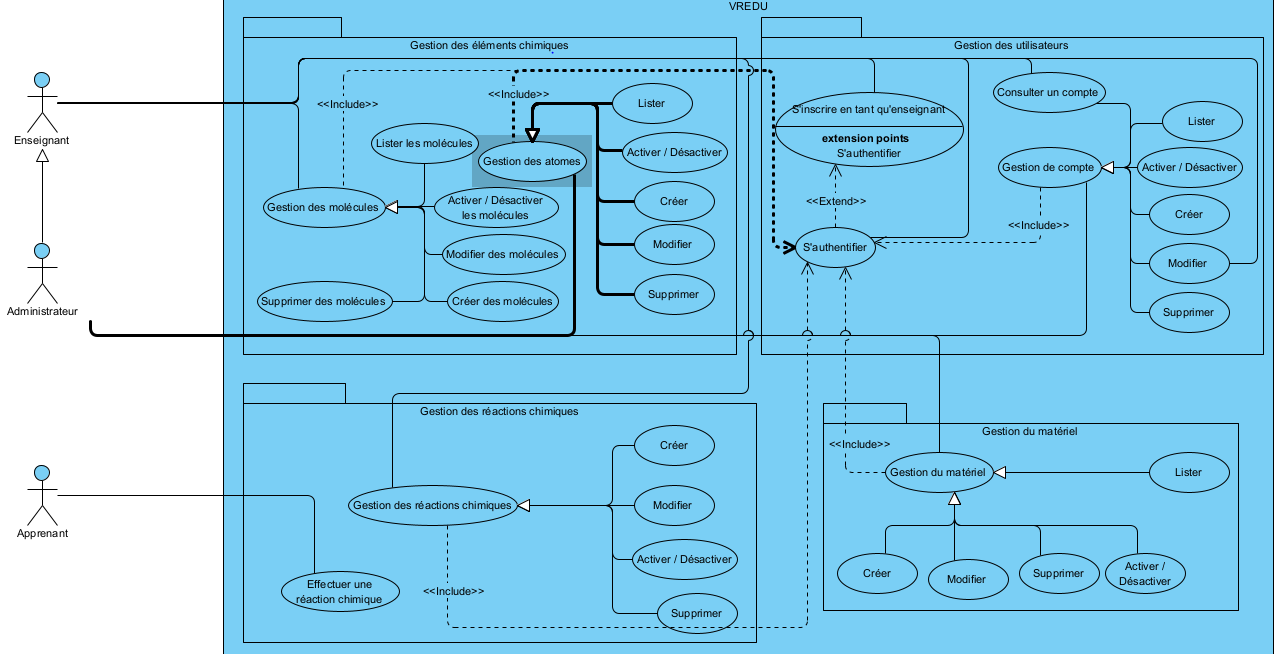
\includegraphics[trim={10cm 0 0 0}, width=1\textwidth]{img/ucd}
	\caption{Diagramme des cas d’utilisation}
	\label{fig:mesh1}
\end{figure}

De ce diagramme ressortent les différents groupe fonctionnalités du module de chimie de l’application VREDU à savoir :  le module de gestion des utilisateurs qui permettra la gestion des compte utilisateur (administrateur et enseignant), le module de gestion des éléments chimique qui permettra les opérations de création, modification. Activation et désactivation des éléments chimiques, le module de gestion des réactions chimiques et le module de gestion du matériel de laboratoire.

\subsubsection{Description textuelle de quelques cas d’utilisation}

\begin{itemize}
	\item \textbf{S’authentifier}
	      \begin{itemize}
		      \item Sommaire d’identification
		            \begin{itemize}
			            \item Titre : s’authentifier
			            \item Acteurs : Administrateur et enseignant
			            \item Objectif : Il permet à l’acteur de s’identifier et se connecter en saisissant son login et mot de passe.
		            \end{itemize}
		      \item Description des scénarios
		            \begin{itemize}
			            \item Précondition : L’acteur doit avoir ouvert l’application
			            \item Post condition :
			                  \begin{itemize}
				                  \item Acteur connecté.
				                  \item Ouverture de l’interface utilisateur.
			                  \end{itemize}
			            \item Scénario nominal
			                  \begin{enumerate}
				                  \item L’acteur demande à ouvrir la page de connexion
				                  \item Le système affiche la page de connexion
				                  \item L’acteur saisit le nom d’utilisateur et son mot de passe
				                  \item Le système vérifie les données
				                  \item Le système connecte l’acteur et affiche l’interface utilisateur
			                  \end{enumerate}
			            \item Scénario alternatif
			                  \begin{itemize}
				                  \item A. Erreur de connexion : nom d'utilisateur ou mot de passe non valide

				                        Cet enchaînement démarre au point 4

				                  \item 5. Le système affiche un message d’erreur correspondant au problème d’identifiants incorrectes.
				                  \item B. Erreur de connexion : le compte est désactivé

				                        Cet enchaînement démarre au point 4

				                  \item 5. Le système affiche un message d’erreur correspondant au problème de compte désactive
			                  \end{itemize}
		            \end{itemize}
	      \end{itemize}
	\item \textbf{Création d’élément chimique }
	      \begin{itemize}
		      \item Sommaire d’identification
		            \begin{itemize}
			            \item Titre : Création d’élément chimique
			            \item Acteurs : Administrateur et enseignant
			            \item Objectif : Il permet à l’acteur de créer un élément chimique pour la plateforme.
		            \end{itemize}
		      \item Description des scénarios
		            \begin{itemize}
			            \item Précondition : Acteur connecté.
			            \item Post condition :
			                  \begin{itemize}
				                  \item Elément chimique crée dans la base de données.
			                  \end{itemize}
			            \item Scénario nominal
			                  \begin{enumerate}
				                  \item L’acteur demande du formulaire de création des éléments
				                  \item Le système affiche le formulaire de création des éléments
				                  \item L’acteur soumet le formulaire de création
				                  \item Le système vérifie les données
				                  \item Le système enregistre l’élément chimique et réinitialise le formulaire
			                  \end{enumerate}
			            \item Scénario alternatif
			                  \begin{itemize}
				                  \item A. Erreur information soumise incorrects

				                        Cet enchaînement démarre au point 4

				                  \item 5. Le système affiche un message d’erreur pour informations soumises incorrect.
			                  \end{itemize}
		            \end{itemize}
	      \end{itemize}

	\item \textbf{Effectuer une réaction}
	      \begin{itemize}
		      \item Sommaire d’identification
		            \begin{itemize}
			            \item Titre : Effectuer une réaction
			            \item Acteurs : Apprenant
			            \item Objectif : Il permet à l’acteur de réaliser une réaction chimique sur la plateforme.
		            \end{itemize}
		      \item Description des scénarios
		            \begin{itemize}
			            \item Précondition : Application ouverte.
			            \item Post condition :
			                  \begin{itemize}
				                  \item L'interface de réalisation des réactions ouverte.
			                  \end{itemize}
			            \item Scénario nominal
			                  \begin{enumerate}
				                  \item L’acteur demande le formulaire d'identification des réactions
				                  \item Le système affiche le formulaire d'identification des réactions
				                  \item L’acteur saisi l'identifiant d'une réaction et soumet le formulaire
				                  \item Le système recherche a réaction
				                  \item Le système envoie de l'interface de réalisation de la réaction
				                  \item L’acteur effectue un mélange et l’envoie
			                  \end{enumerate}
			            \item Scénario alternatif
			                  \begin{itemize}
				                  \item A. Erreur réaction introuvable.

				                        Cet enchaînement démarre au point 4

				                  \item 5.  Le système affiche un message d’erreur pour réaction introuvable.
				                  \item B. Erreur réaction désactivée
				                  \item 5. Le système affiche un message d’erreur pour réaction désactivée
			                  \end{itemize}
		            \end{itemize}
	      \end{itemize}

	\item \textbf{Création d’une réaction}
	      \begin{itemize}
		      \item Sommaire d’identification
		            \begin{itemize}
			            \item Titre : Création d’une réaction
			            \item Acteurs : Administrateur et enseignant
			            \item Objectif : Il permet à l’acteur de créer une réaction chimique pour la plateforme.
		            \end{itemize}
		      \item Description des scénarios
		            \begin{itemize}
			            \item Précondition : Acteur connecté.
			            \item Post condition :
			                  \begin{itemize}
				                  \item Réaction chimique crée dans la base de données.
			                  \end{itemize}
			            \item Scénario nominal
			                  \begin{enumerate}
				                  \item L’acteur demande à créer une réaction
				                  \item Le système retourne le formulaire de création
				                  \item L’acteur envoie les informations sur la réaction
				                  \item Le système demande une confirmation de création.
				                  \item L’acteur confirme la création
				                  \item Le système enregistre la réaction
			                  \end{enumerate}
			            \item Scénario alternatif
			                  \begin{itemize}
				                  \item A. L’acteur annule la création

				                        Cet enchaînement démarre au point 4

				                  \item 5. Le système annule la création.

				                        Le scénario reprend au point 3
			                  \end{itemize}
		            \end{itemize}
	      \end{itemize}

	\item \textbf{Suppression d’une réaction }
	      \begin{itemize}
		      \item Sommaire d’identification
		            \begin{itemize}
			            \item Titre : Suppression d’une réaction
			            \item Acteurs : Administrateur et enseignant
			            \item Objectif : Il permet à l’acteur de supprimer une réaction sur la plateforme.
		            \end{itemize}
		      \item Description des scénarios
		            \begin{itemize}
			            \item Précondition : Acteur connecté.
			            \item Post condition :
			                  \begin{itemize}
				                  \item La réaction est supprimée de la base de données de l’application.
			                  \end{itemize}
			            \item Scénario nominal
			                  \begin{enumerate}
				                  \item L’acteur demande de la liste des réactions
				                  \item Le système retourne la liste des réactions
				                  \item L’acteur sélectionne une réaction
				                  \item Le système demande une confirmation de suppression.
				                  \item L’acteur confirme la suppression
				                  \item Le système supprime la réaction
			                  \end{enumerate}
			            \item Scénario alternatif
			                  \begin{itemize}
				                  \item A. L’acteur annule la suppression

				                        Cet enchaînement démarre au point 4

				                  \item 5. Le système annule la suppression.

				                        Le scénario reprend au point 3
			                  \end{itemize}
		            \end{itemize}
	      \end{itemize}
\end{itemize}

\subsubsection{Diagrammes de séquences}

Les diagrammes de séquences sont la représentation graphique des interactions entre les acteurs et le système selon un ordre chronologique.

\begin{itemize}
	\item \textbf{S’authentifier}

	      \begin{figure}[H]
		      \centering
		      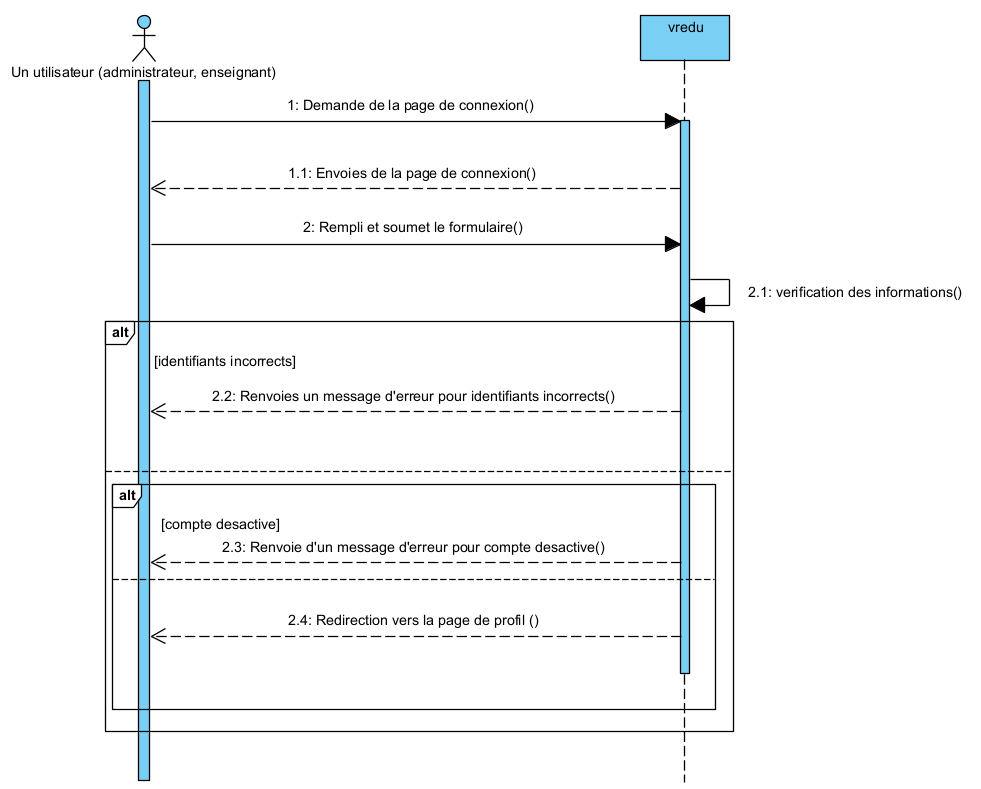
\includegraphics[width=1\textwidth]{img/ucdAuth}
		      \caption{Diagrammes de séquences du cas d'utilisation s’authentifier}
		      \label{fig:mesh1}
	      \end{figure}

	      Ce diagramme fait une description détaille du cas d’utilisation d’authentification qui permet à un utilisateur d’être reconnue par le système afin de lui accorder certain droit sur le système en fonction de son identité.


	\item \textbf{Création d’élément chimique}

	      \begin{figure}[H]
		      \centering
		      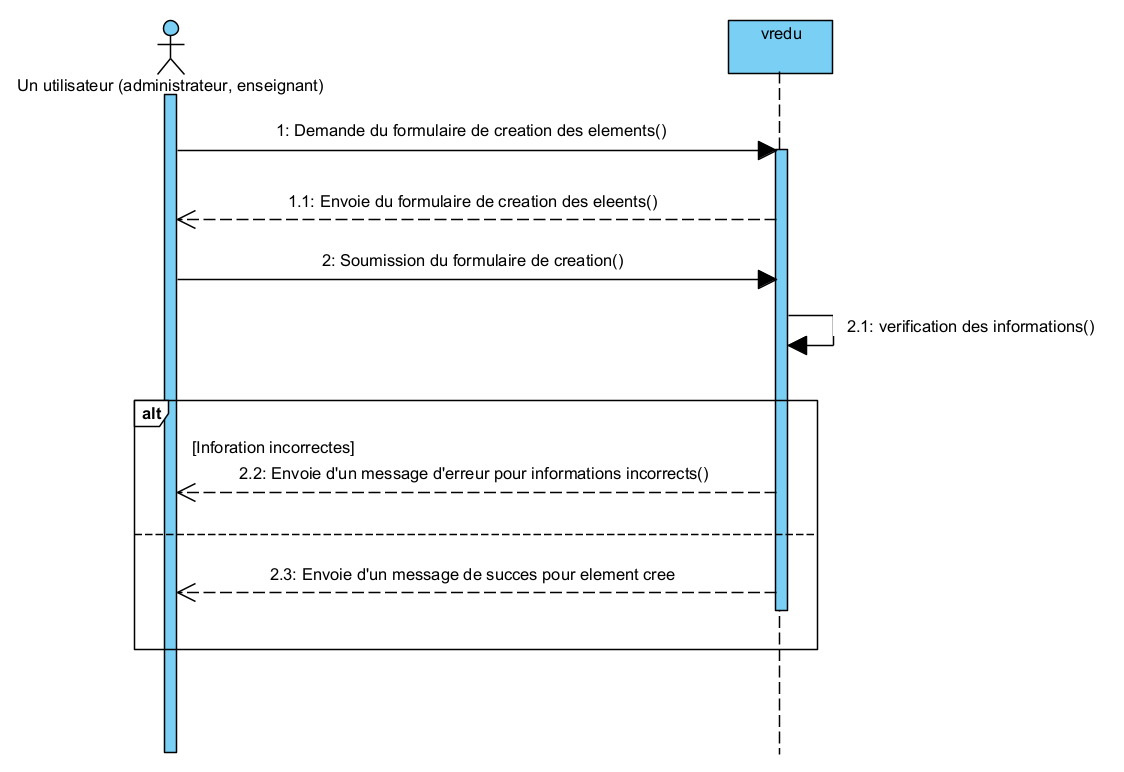
\includegraphics[width=1\textwidth]{img/ucdElCr}
		      \caption{Diagrammes de séquences du cas d'utilisation création d’élément chimique}
		      \label{fig:mesh1}
	      \end{figure}

	      Ce diagramme fait une description détaille du cas d’utilisation création d’un élément chimique, ce cas permet à un utilisateur connecte de créer un élément chimique pour une réaction chimique.


	\item \textbf{Effectuer une réaction}

	      \begin{figure}[H]
		      \centering
		      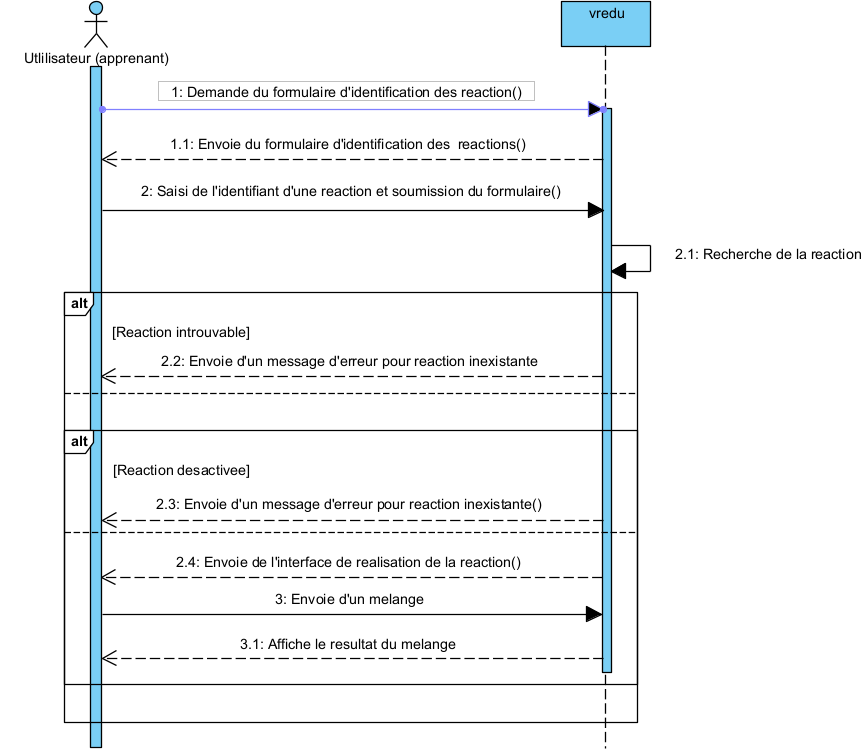
\includegraphics[width=1\textwidth]{img/ucdeur}
		      \caption{Diagrammes de séquences du cas d'utilisation effectuer une réaction}
		      \label{fig:mesh1}
	      \end{figure}

	      Ce diagramme fait une description détaille du cas effectuer une réaction qui présente le processus de réalisation d’une réaction chimique sur le système par un apprenant.
\end{itemize}

\subsubsection{Diagrammes d’activités}

Les diagrammes d'activités permettent de mettre l'accent sur les traitements. Ils sont donc particulièrement adaptés à la modélisation du cheminement de flots de contrôle et de flots de données. Ils permettent ainsi de représenter graphiquement le comportement d'une méthode ou le déroulement d'un cas d'utilisation.

\begin{itemize}
	\item \textbf{Créer une réaction }

	      \begin{figure}[H]
		      \centering
		      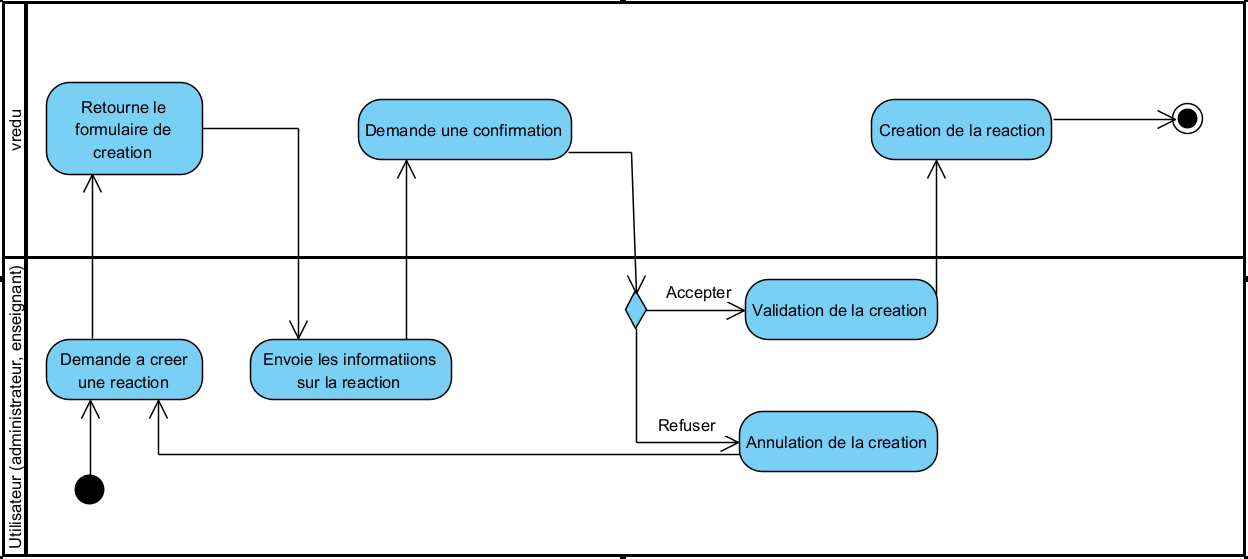
\includegraphics[width=1\textwidth]{img/sdCUR}
		      \caption{Diagrammes d’activités du cas d'utilisation créer une réaction}
		      \label{fig:mesh1}
	      \end{figure}

	      Ce diagramme fait une description détaille du cas créer une réaction qui présente le processus de création d’une réaction chimique sur le système par un administrateur ou un enseignant.

	\item \textbf{Suppression d’une réaction}

	      \begin{figure}[H]
		      \centering
		      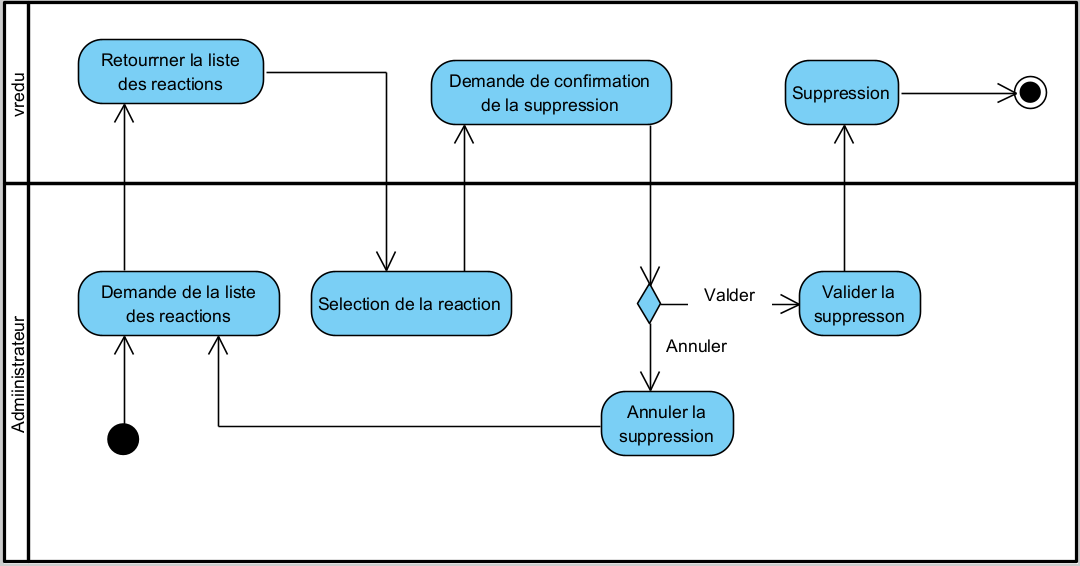
\includegraphics[width=1\textwidth]{img/adsr}
		      \caption{Diagrammes d’activités du cas d'utilisation suppression d’une réaction}
		      \label{fig:mesh1}
	      \end{figure}

	      Ce diagramme fait une description détaille du cas suppression d’une réaction qui présente le processus de suppression d’une réaction chimique sur le système par un administrateur ou un enseignant.
\end{itemize}

\subsubsection{Diagramme d’état transition}

Un diagramme d'états-transitions est un type de diagramme comportemental en langage de modélisation unifié (UML) qui représente les transitions entre divers objets.

\begin{itemize}
	\item \textbf{Changement d’état des produits d’une réaction}

	      \begin{figure}[H]
		      \centering
		      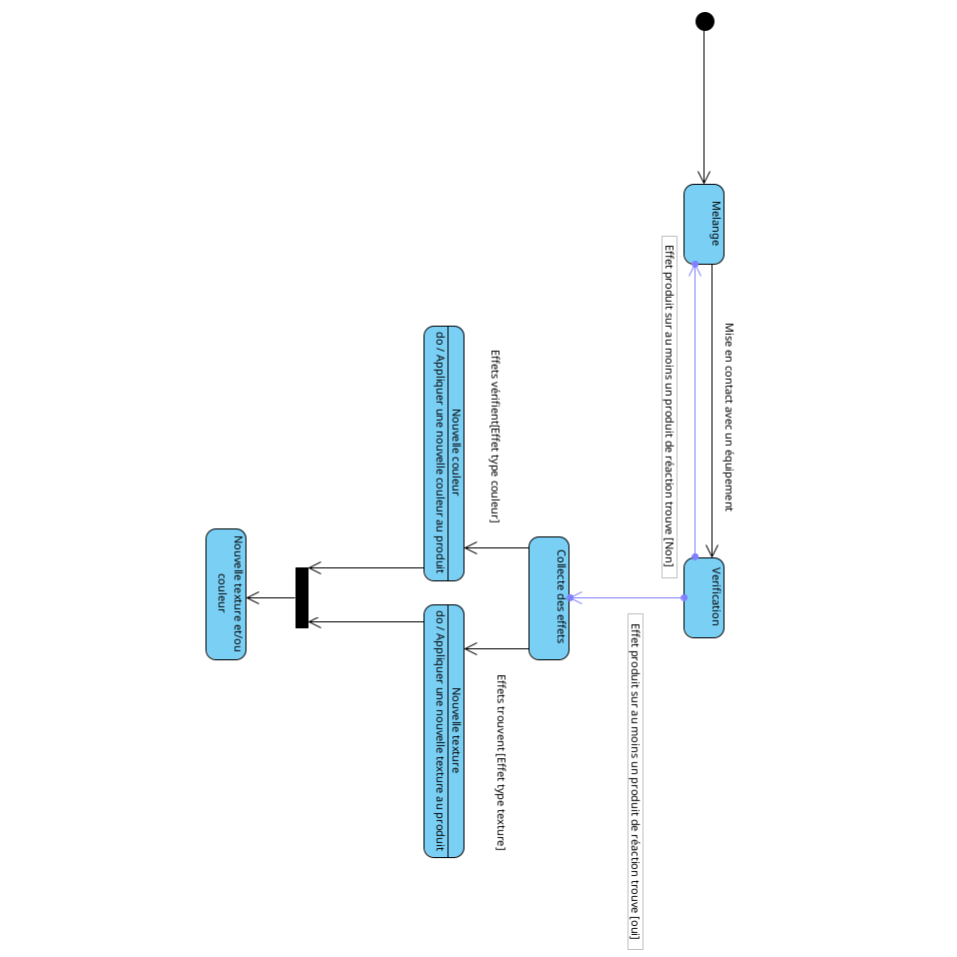
\includegraphics[width=1\textwidth]{img/etdR}
		      \caption{Diagramme d’état transition du cas d'utilisation changement d’état des produits d’une réaction}
		      \label{fig:mesh1}
	      \end{figure}

	      Ce diagramme présente de façon détaillée le processus de changement d’état d’un produit de réaction lors d’une réaction chimique.

	\item \textbf{Changement d’état d'authentification d’un utilisateur }

	      \begin{figure}[H]
		      \centering
		      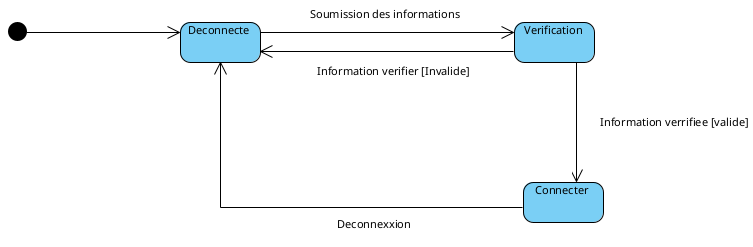
\includegraphics[width=1\textwidth]{img/etu}
		      \caption{Diagramme d’état transition du cas d'utilisation changement d’état d'authentification d’un utilisateur}
		      \label{fig:mesh1}
	      \end{figure}

	      Ce diagramme présente de façon détaillée le changement d’état d’authentification d’un utilisateur en fonction d’évènement effectues sur la plateforme.
\end{itemize}

\subsection{Analyse non fonctionnelle} % (fold)

C’est l’ensemble des exigences qui ne concernent pas spécifiquement le comportement du système mais plutôt identifient des contraintes internes et externes du système. Ainsi les principaux besoins non fonctionnels de notre système sont :

\begin{itemize}
	\item Le code doit être clair, bien structuré pour permettre des futures évolutions du système ;
	\item L’ergonomie : la plateforme doit offrir des interfaces conviviales et faciles à utiliser ;
\end{itemize}

\subsection{Technique et Méthodes} % (fold)

\subsubsection{Choix des techniques de développement}

Plusieurs techniques peuvent être utilisées pour réaliser d’une plateforme web et 3D :

\begin{itemize}
	\item \textbf{Le code pur et dur} :

	      C’est ainsi que les informaticiens créent leur première application. Il est nécessaire d’avoir de bonnes connaissances en programmation. En effet toute l'application est créée à partir de ligne de code complètement illisible pour un profane. Cette solution est longue, couteuse et rarement assez complète pour permettre une modification facile de l’application. Aujourd’hui, la plupart des développeurs ne crée plus leur application de A à Z, ils utilisent une des méthodes suivantes.

	\item \textbf{Les CMS (Content management system) pour le web} :

	      Ce sont des aides à la création d’applications. Ils ne font pas tous à votre place, mais vous aident en grande partie. Il est très recommandé d’avoir des connaissances en informatique pour réaliser une application à partir d’un CMS. Certains sont en effet très compliqués à mettre en place. De plus aucun hébergement n’est fourni avec le CMS. Il faudra donc mettre en place un serveur HTTP pour héberger son application. Pour finir, la personnalisation du design d’une application sur un CMS est assez fastidieuse. Il sera presque à tous les cas obligatoires de mettre la main dans le code source de   l’application. D’autres techniques existent notamment les Outils en ligne.

	\item \textbf{Framework et librairies} :

	      Il existe également des Framework et librairies (bout de code écrit permettant de faciliter le travail du développeur), qui est l’une des méthodes les plus utilisée dans le monde du développement, nous avons donc optes pour cette méthode et nous allons choisir un Framework parmi ceux existant.
\end{itemize}

\subsubsection{Choix du Framework}

\textbf{ASP.net} pour le \textbf{backend}, \textbf{React} pour le \textbf{frontend} et \textbf{unreal engine} pour la \textbf{3D}. Comme \textbf{SGBD}, nous avons allons utiliser \textbf{PostgreSQL} (le SGBD utilisé par l’entreprise).

\section{Conception du système}

\subsection{Diagramme de classe} % (fold)

Le diagramme de classes est un schéma utilisé pour présenter les classes et les interfaces des systèmes ainsi que leurs relations.

\begin{figure}[H]
	\centering
	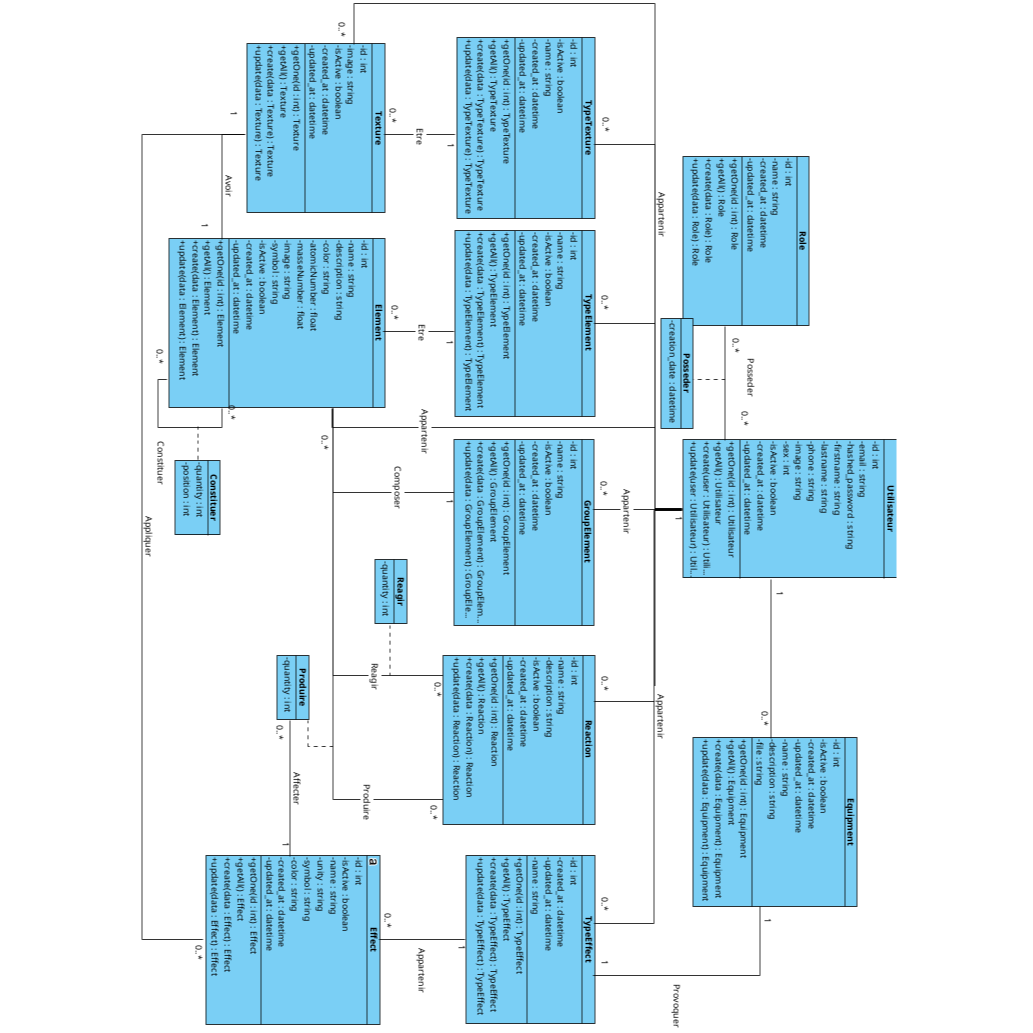
\includegraphics[trim={5cm 0 0 0}, width=1\textwidth]{img/dc}
	\caption{Diagramme de classe du système}
	\label{fig:mesh1}
\end{figure}

Ce diagramme présente les classes et leurs interactions dans le système.

\subsection{Diagramme de déploiement} % (fold)

En UML, un diagramme de déploiement est une vue statique qui sert à représenter l’utilisation de l’infrastructure physique par le système et la manière dont les composants du système sont répartis ainsi que leurs relations entre eux. Les éléments utilisés par un diagramme de déploiement sont principalement les nœuds, les composants, les associations et les artefacts. Les caractéristiques des ressources matérielles physiques et des supports de communication peuvent être précisées par stéréotype.

\begin{figure}[H]
	\centering
	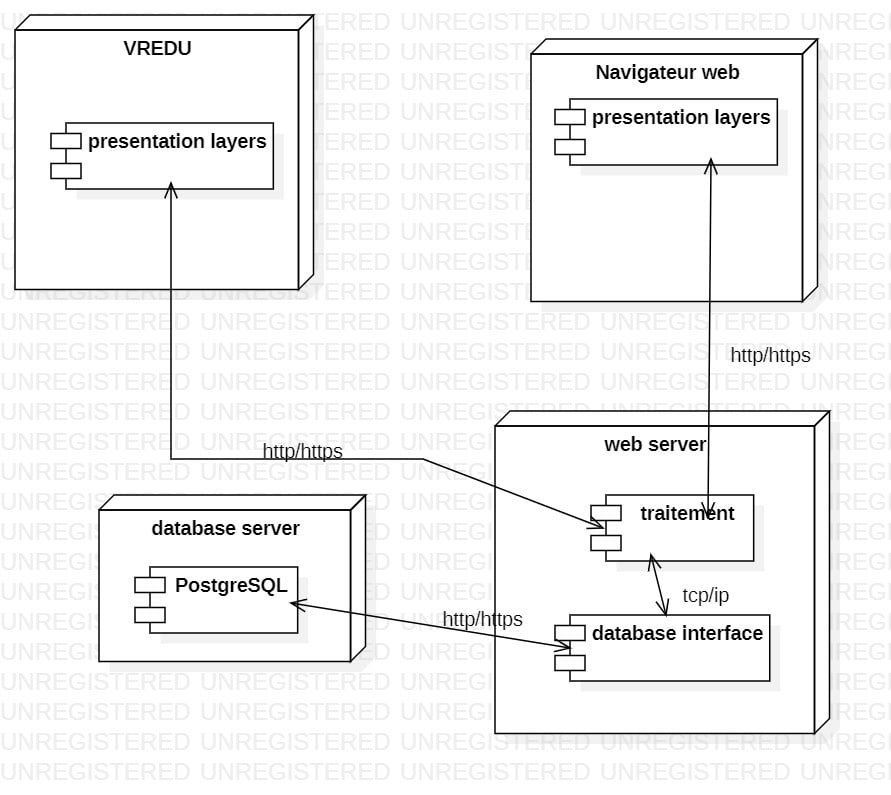
\includegraphics[width=1\textwidth]{img/dd}
	\caption{Diagramme de déploiement du système}
	\label{fig:mesh1}
\end{figure}

\subsection{Quelques maquettes d'IHM (Interface Homme Machine)}

\subsubsection{Page d'accueil}

Cette page de décrire la solution aux enseignants qui souhaites la découvrir.

\begin{figure}[H]
	\centering
	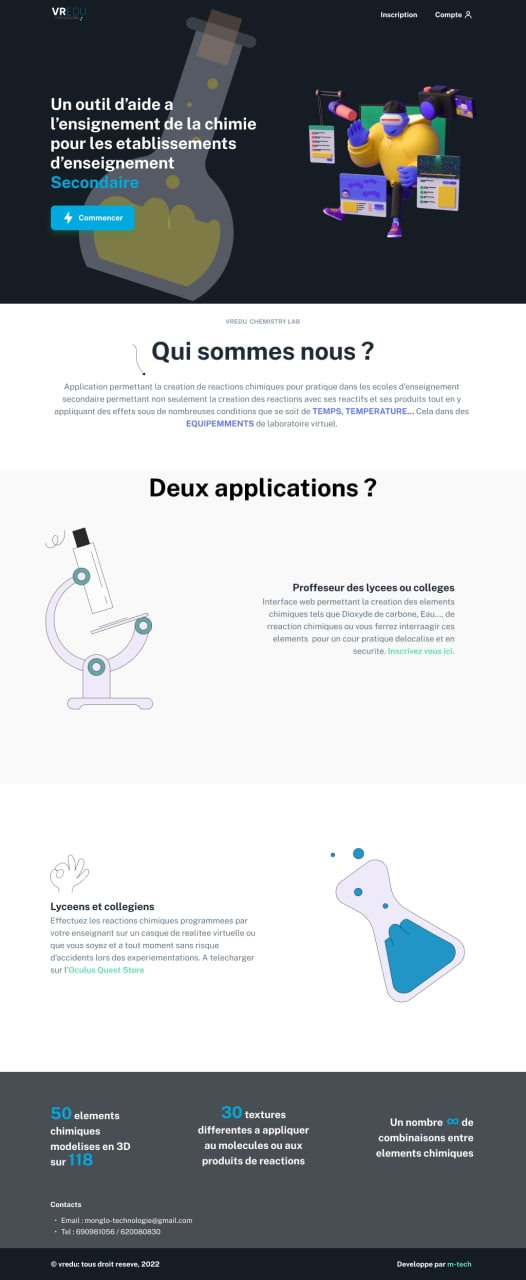
\includegraphics[width=0.5\textwidth]{img/home}
	\caption{IHM de la page d'accueil}
	\label{fig:mesh1}
\end{figure}

Il y apparait clairement une entête de page avec le logo et les différents liens d'inscription et de connexion.
Les sections suivantes décrivent la solutions, présentent ses statistiques et les contacts en cas de questions ou de problèmes.

\subsubsection{Page d'inscription des enseignants}

Cette page permet la création de compte enseignant en y renseignant les informations personnelles de l'utilisateur.

\begin{figure}[H]
	\centering
	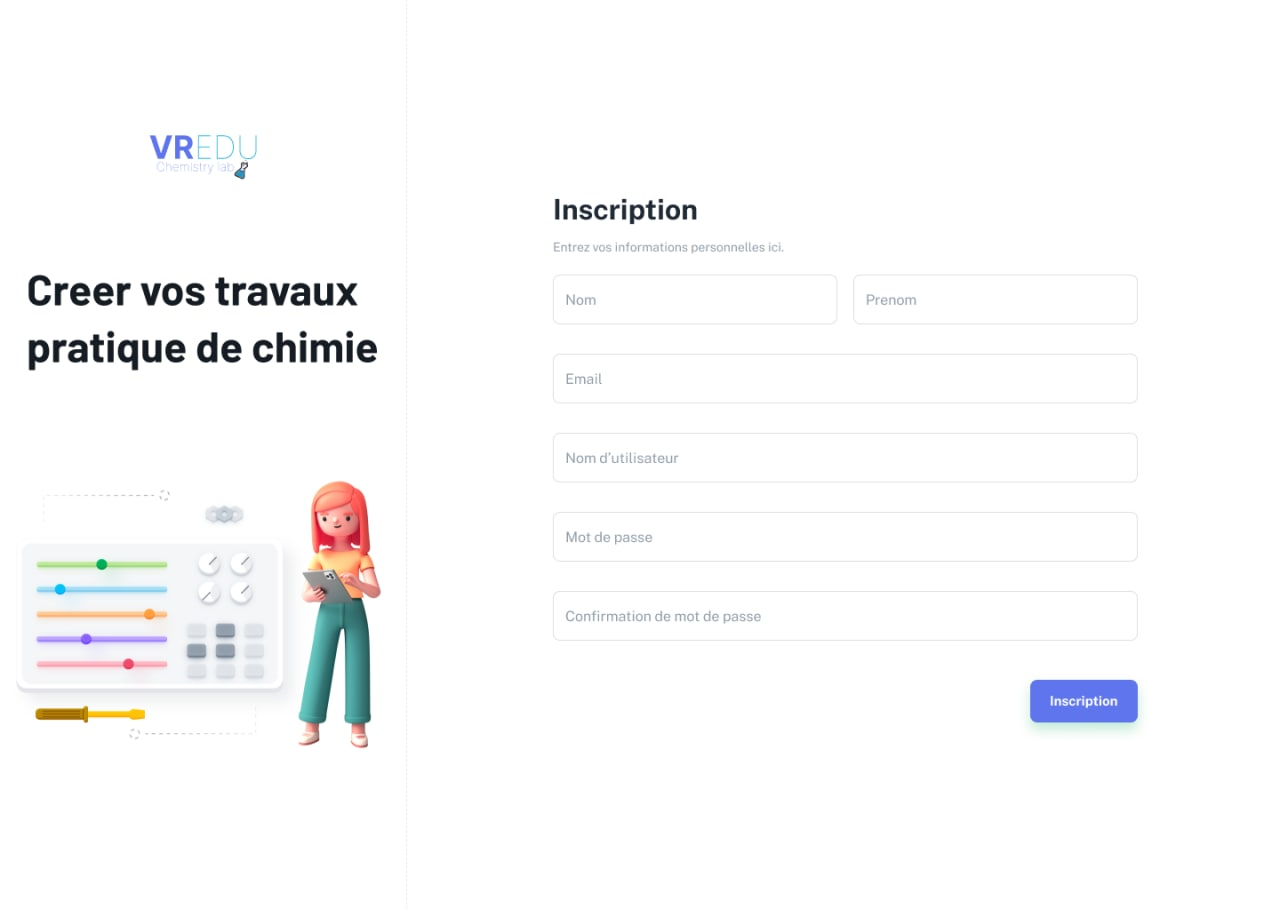
\includegraphics[width=1\textwidth]{img/insc}
	\caption{IHM de la page d'inscription des enseignants}
	\label{fig:mesh1}
\end{figure}

Il y apparait le formulaire de création de compte avec les différents champs remplir avant la soumission.

\subsubsection{Page de connexion des enseignants}

Cette page permet à tous les utilisateurs d’accéder à l’application en utilisant un login et
un mot de passe.

\begin{figure}[H]
	\centering
	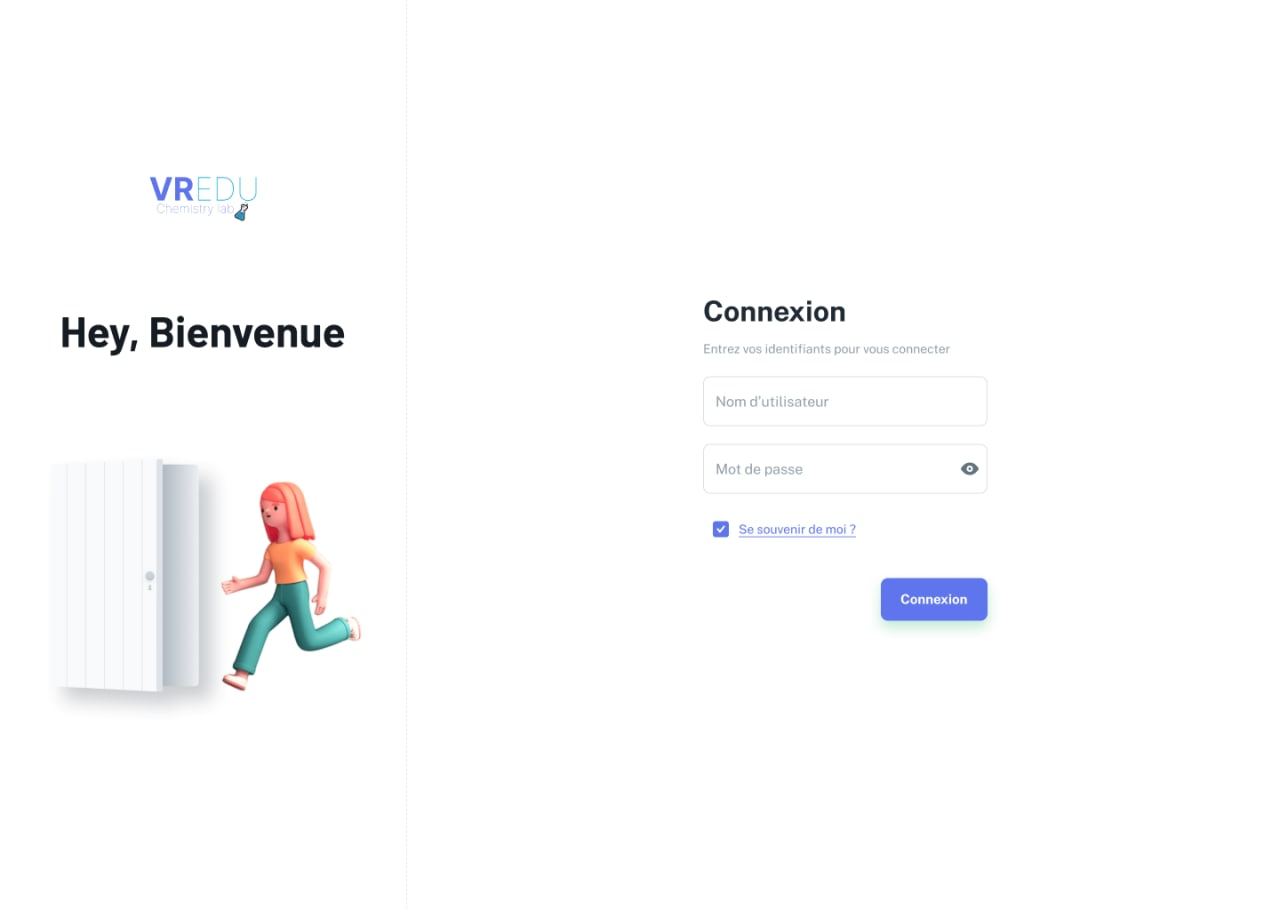
\includegraphics[width=1\textwidth]{img/conn}
	\caption{IHM de la page de connexion des enseignants}
	\label{fig:mesh1}
\end{figure}

Il y apparait le formulaire de connexion avec les champs pour le nom d'utilisateur et le mot de passe à remplir avant soumission.
Deux catégorie d'utilisateurs peuvent utiliser cette interface à savoir les administrateurs et les enseignants.

\subsubsection{Page espace personnel des enseignants et administrateurs}

Cette page permet à l'utilisateur d'avoir un appercu de ses réactions.

\begin{figure}[H]
	\centering
	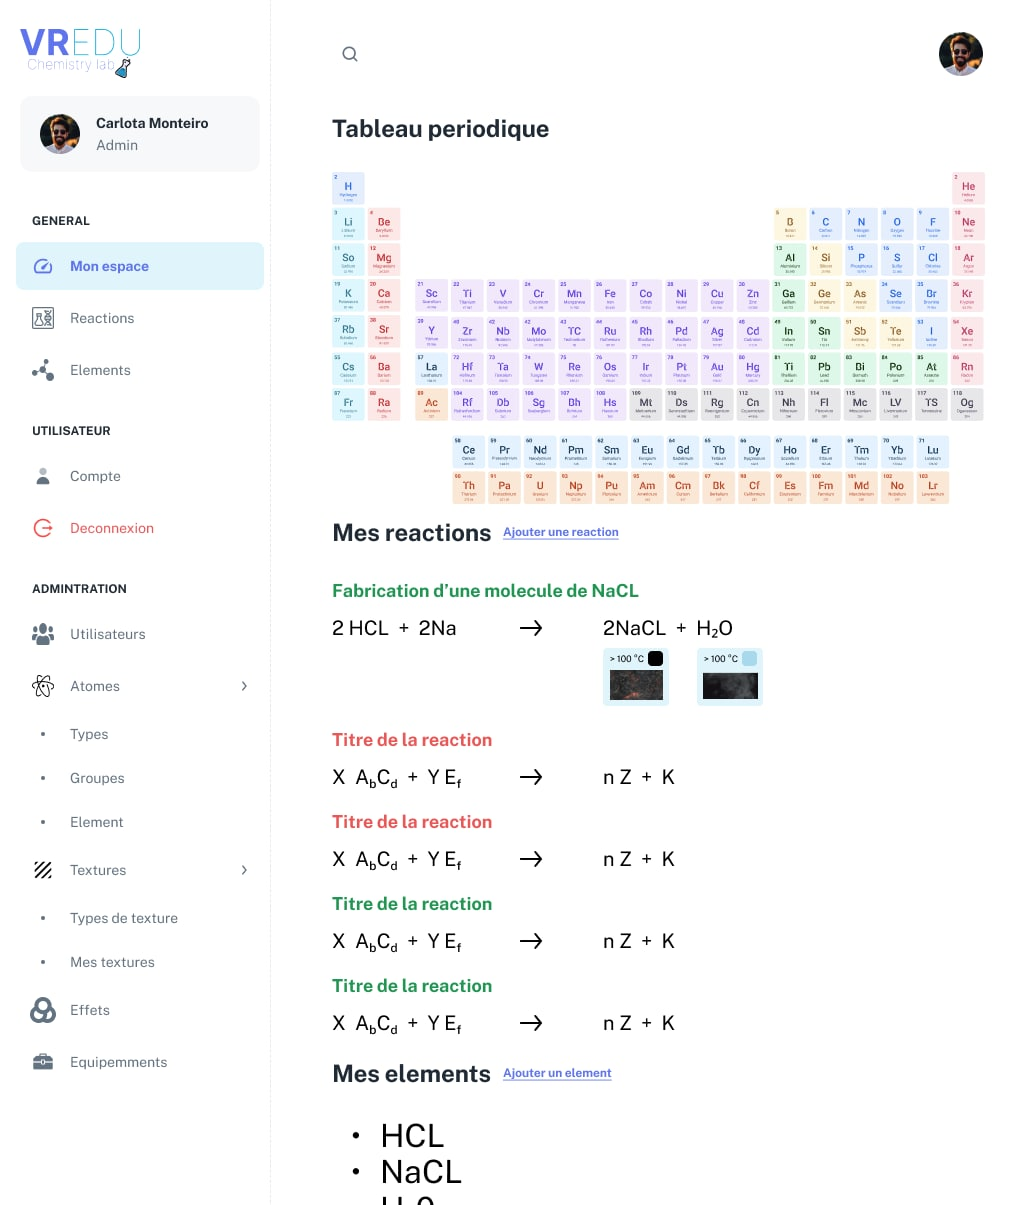
\includegraphics[width=1\textwidth]{img/esp}
	\caption{IHM de la page espace personnel des enseignants et administrateurs}
	\label{fig:mesh1}
\end{figure}

Il y apparait la liste des éléments chimiques du tableau périodique et la liste des réactions de l'utilisateur connecté.

\subsubsection{Interface du laboratoire en vue de dessus}

Cette interface représente une vue de dessus du laboratoire virtuelle ou les apprenant effectuerons leur réactions.

\begin{figure}[H]
	\centering
	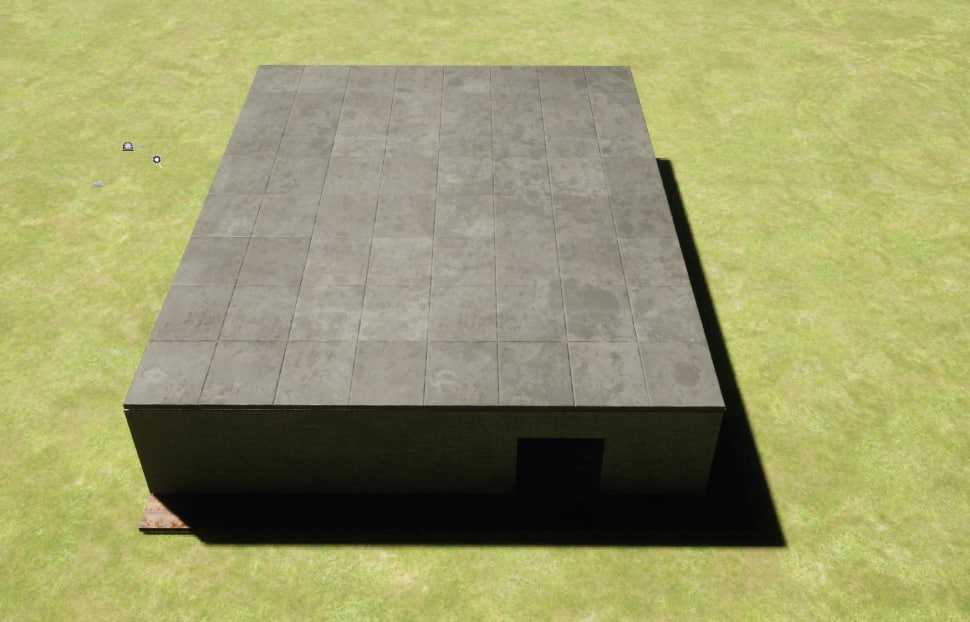
\includegraphics[width=1\textwidth]{img/labot}
	\caption{IHM du laboratoire en vue de dessus}
	\label{fig:mesh1}
\end{figure}

Il y apparait un locale vue du dessus et présente l'environnement extérieur du laboratoire oû aurons lieu les réactions.

\subsubsection{Interface du laboratoire en vue de face}

Cette interface représente une vue de face du laboratoire virtuelle ou les apprenant effectuerons leur réactions.

\begin{figure}[H]
	\centering
	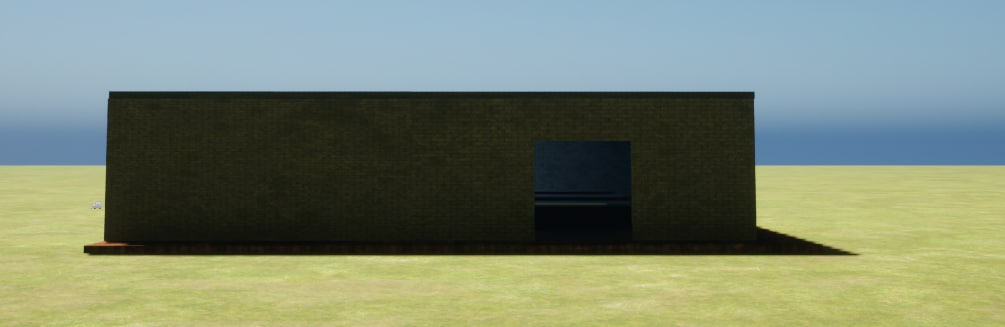
\includegraphics[width=1\textwidth]{img/labof}
	\caption{IHM du laboratoire en vue de face}
	\label{fig:mesh1}
\end{figure}

Il y apparait un locale vue de face et présente l'environnement extérieur du laboratoire oû aurons lieu les réactions.

\subsubsection{Interface du laboratoire intérieur vue du fond}

Cette interface représente une vue interieur du laboratoire vu du fond de la salle.

\begin{figure}[H]
	\centering
	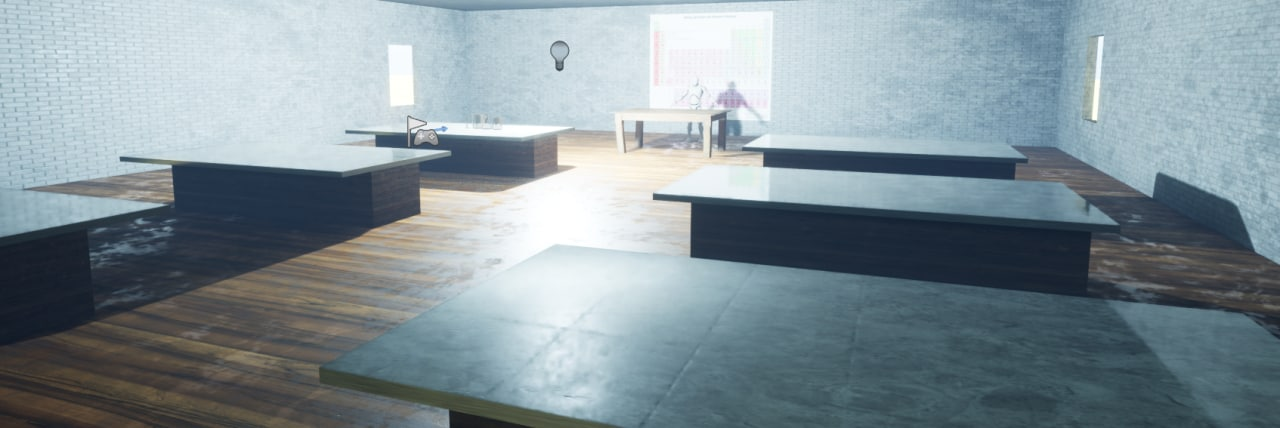
\includegraphics[width=1\textwidth]{img/labo1}
	\caption{IHM du laboratoire intérieur vue du fond}
	\label{fig:mesh1}
\end{figure}

Il y apparait une vue du locale et est présenté l'environnement intérieur du laboratoire avec les tables ou se déroulerons les réactions.

\subsubsection{Interface du laboratoire intérieur vue de l'apprenant}

Cette interface représente le point de vue d'un apprenant qui utilise l'application.

\begin{figure}[H]
	\centering
	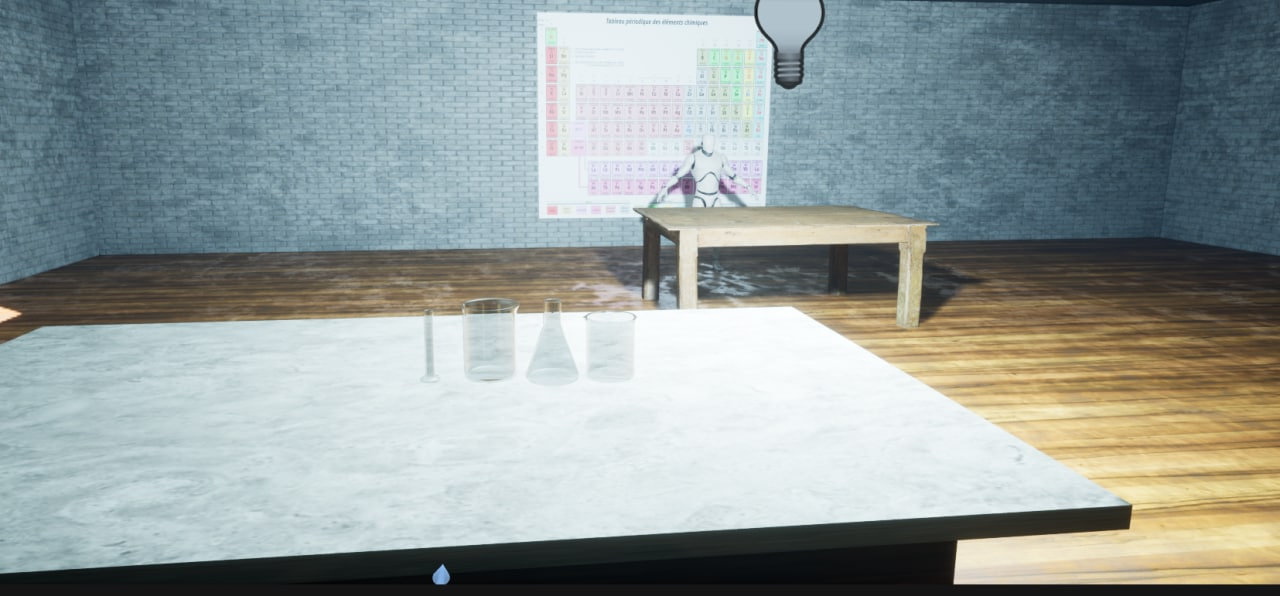
\includegraphics[width=1\textwidth]{img/labo2}
	\caption{IHM du laboratoire intérieur vue de l'apprenant}
	\label{fig:mesh1}
\end{figure}

Il y apparait la table de l'apprenant avec la verrerie des réaction disposé dessus.

\subsubsection{Interface du laboratoire intérieur vue de l'enseignant}

Cette interface représente le point de vue d'un enseignant qui utilise l'application.

\begin{figure}[H]
	\centering
	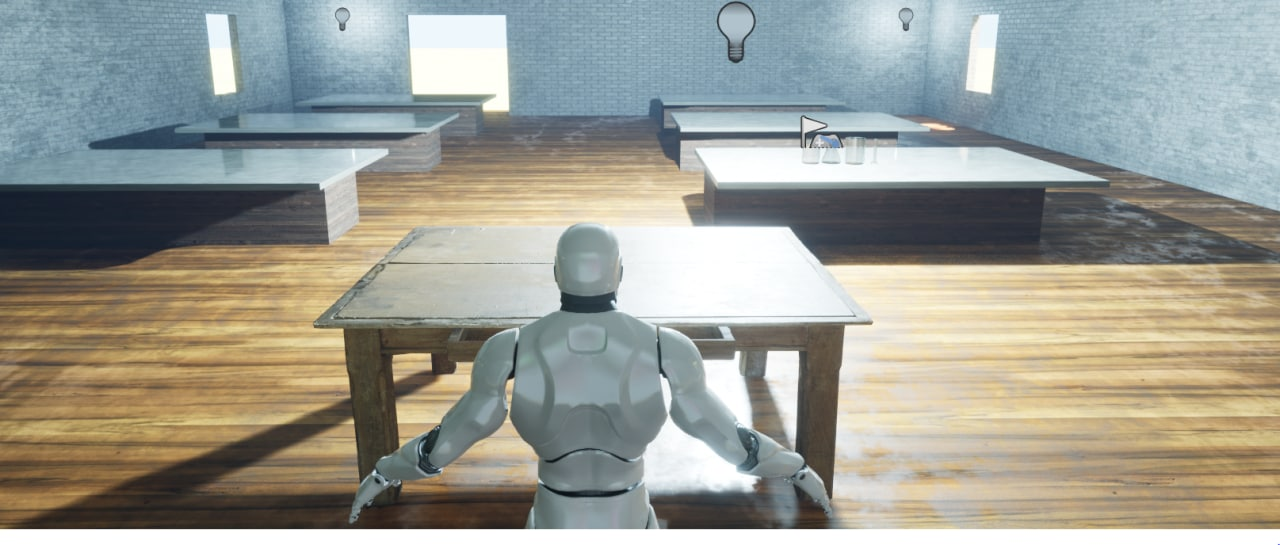
\includegraphics[width=1\textwidth]{img/labo3}
	\caption{IHM du laboratoire intérieur vue de l'enseignant}
	\label{fig:mesh1}
\end{figure}

Il y apparait les tables de réaction des différents apprenants dans le laboratoire virtuel.


\chapter{Implémentation de la solution et résultats}
\textit{Dans ce chapitre, nous ferons un tour d’horizon sur l’ensemble des technologies utilisées
	afin de mettre en œuvre la solution et montrerons comment nous comptons déployer notre
	solution. Enfin nous présenterons quelques résultats obtenus par implémentation.}
\clearpage

\section{Outils et technologies}

De la conception à la réalisation de notre application, nous avons eu à utiliser les outils et technologies suivants :

\begin{itemize}
	\item \textbf{Unreal Engine 5} : qui est un moteur de rendu 3D utilisé dans la création de jeux et la simulation d'environnement 3D utilisant le langage de programmation c++.
	\item \textbf{React \& React Dom} : qui est un Framework javascript très populaire permettant la création d’interfaces utilisateur web simplement et rapidement, il offre une grande documentation et possède une communauté très active.
	\item \textbf{ASP.NET core web api} : est un Framework C\# permettant la création d’api REST développé par Microsoft.
	\item \textbf{PostgreSQL} : C’est un système de gestion de base de données relationnelle et objet. C'est un outil libre disponible selon les termes d'une licence de type BSD. Ce système est concurrent d'autres systèmes de gestion de base de données, qu'ils soient libres, ou propriétaires ;
	\item \textbf{Git \& GitHub} : Git est un logiciel de gestion de versions décentralisé. C'est un logiciel libre créé par Linus Torvalds, auteur du noyau Linux, et distribué selon les termes de la licence publique générale GNU version 2. GitHub est un logiciel libre de forge basé sur git proposant les fonctionnalités de wiki, un système de suivi des bugs, l’intégration continue et la livraison continue ;
	\item \textbf{Rider} : C’est un environnement de développement .NET multiplateforme de chez jetbrains basé sur la plateforme IntelliJ et ReSharper.
	\item \textbf{Webstorm} : C’est un IDE pour les langages Web, développé par l'entreprise JetBrains et basé sur la plateforme IntelliJ IDEA ;
	\item \textbf{Docker} : C’est un IDE pour les langages Web, développé par l'entreprise JetBrains et basé sur la plateforme IntelliJ IDEA ;
	\item \textbf{Jira} : est un système de suivi de bugs, de gestion des incidents et de gestion de projets développé par Atlassian.
	\item \textbf{Visual paradigme} : C’est un outil UML CASE prenant en charge UML 2, SysML et la notation de modélisation de processus métier (BPMN) d’Object Management Group (OMG). Outre la modélisation, il offre des fonctionnalités de génération de rapports et d’ingénierie de code, y compris la génération de code.
	\item \textbf{Gantt Project} : est un logiciel libre de gestion de projet écrit en Java.
\end{itemize}

\section{Résultats}

\subsection{Édition du profile utilisateur}

\subsubsection{Interface d'édition du profile utilisateur}

Il est question de l'interface qui permettra à un utilisateur en occurence un administrateur ou un enseignant de modifier ses information personnelles.

\begin{figure}[H]
	\centering
	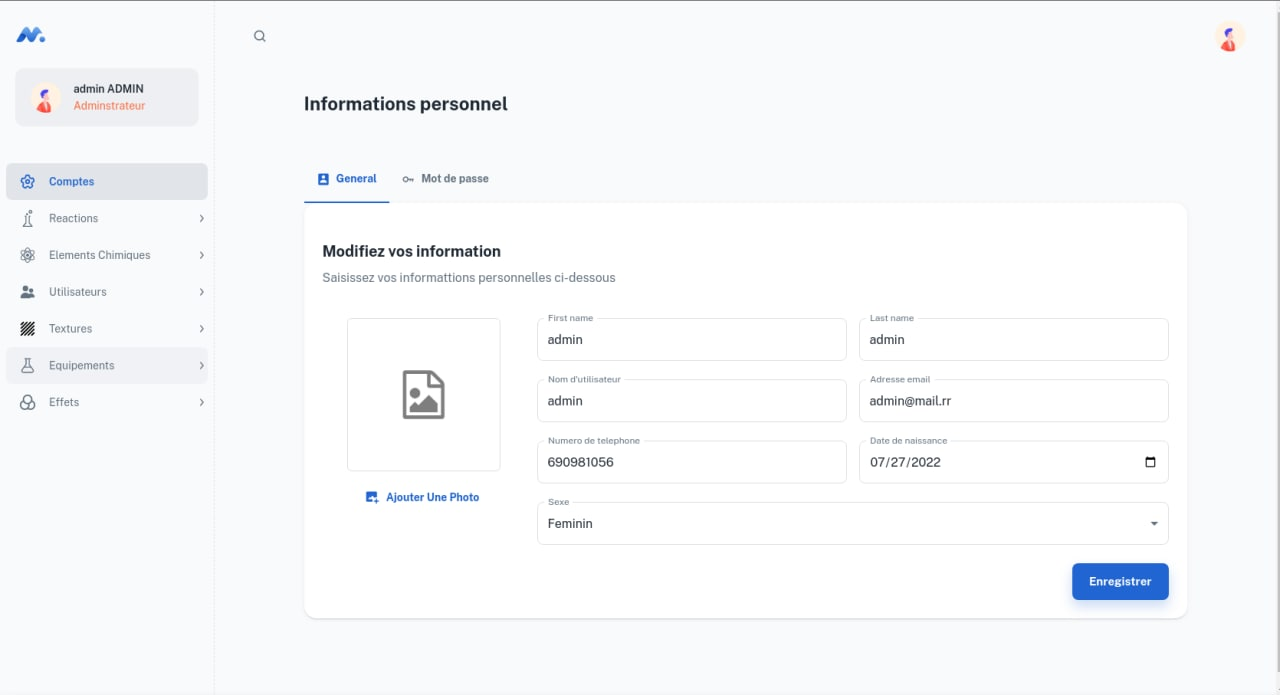
\includegraphics[width=1\textwidth]{img/editpr}
	\caption{IHM formulaire d'édition du profile utilisateur}
	\label{fig:mesh1}
\end{figure}

Il y apparait à gauche les différents menus disponibles de l'application, et à gauche une zone de fomulaire permettant la modification des informations d'un utilisateur.

\subsubsection{Code source backend}

\begin{figure}[H]
	\centering
	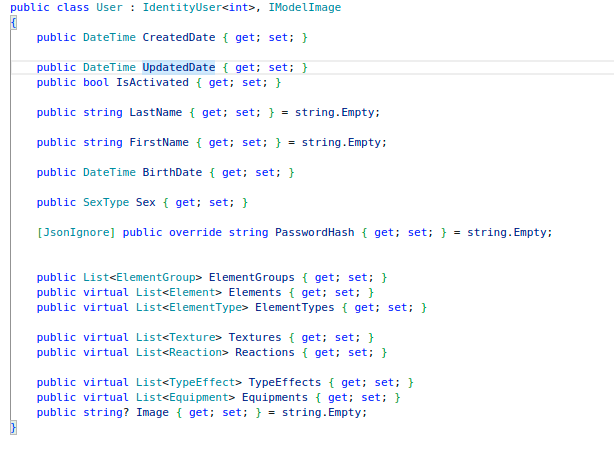
\includegraphics[width=1\textwidth]{img/codeuu}
	\caption{Code backend du model d'utilisateur}
	\label{fig:mesh1}
\end{figure}

Il est question ici de la définition du model d'utilisateur qui sera stocké en base de données.

\begin{figure}[H]
	\centering
	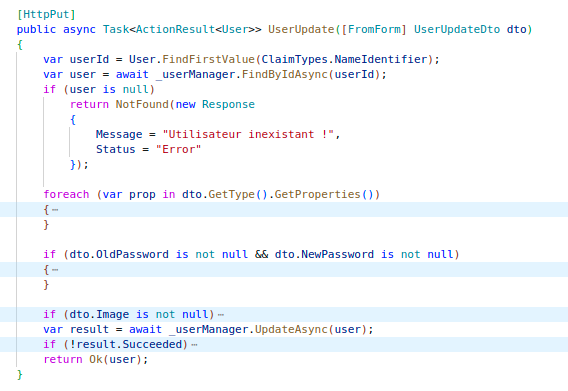
\includegraphics[width=1\textwidth]{img/codeuup}
	\caption{Code backend du cas d'utilisation de l'édition du profile utilisateur}
	\label{fig:mesh1}
\end{figure}

Il est question ici d'une partie du code du controller permettant la gestion des utilisateurs avec la fonctionnalités d'édition des comptes utilisateurs.

\begin{figure}[H]
	\centering
	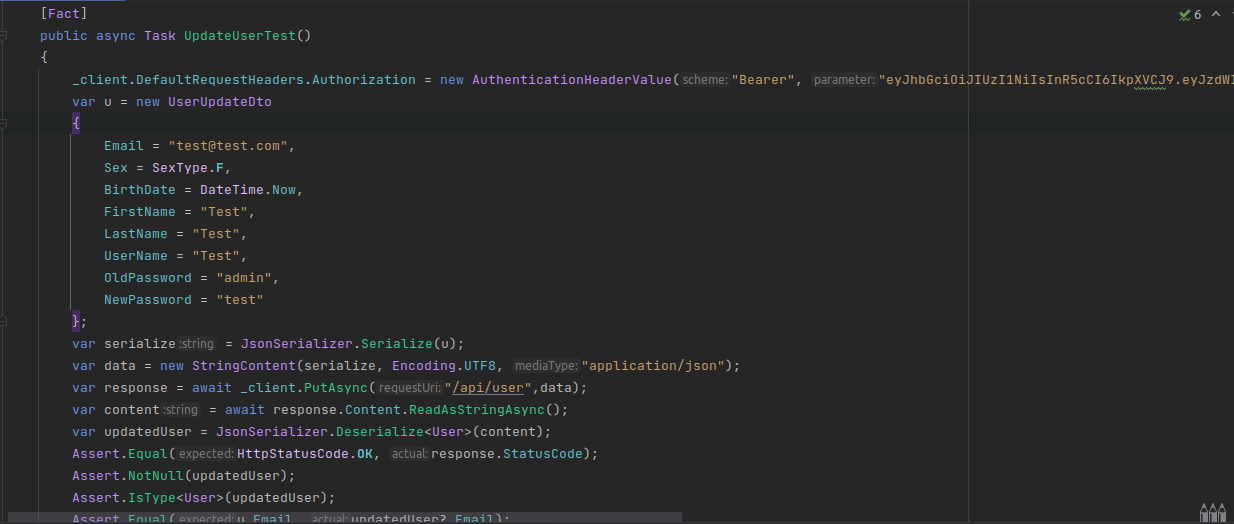
\includegraphics[width=1\textwidth]{img/utupdate}
	\caption{Code backend du test unitaire du cas d'utilisation de l'édition du profile utilisateur}
	\label{fig:mesh1}
\end{figure}

Il est question ici d'une partie du code de test de la fonctionnalités d'édition du profile utilisateur.

\begin{figure}[H]
	\centering
	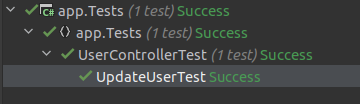
\includegraphics[width=1\textwidth]{img/uutr}
	\caption{Résultat du test unitaire du cas d'utilisation de l'édition du profile utilisateur}
	\label{fig:mesh1}
\end{figure}

Nous avons ici le resultat du test unitaire du cas d'utilisation de l'édition du profile utilisateur, qui s'avère concluent.

\subsubsection{Code source frontend}

\begin{figure}[H]
	\centering
	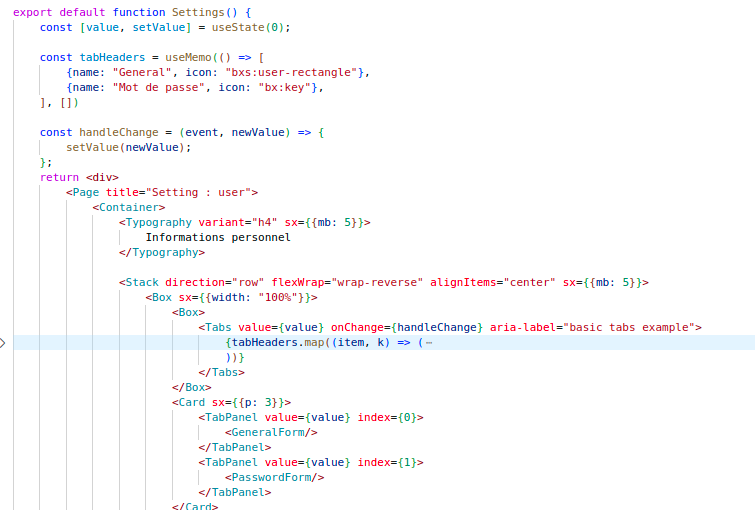
\includegraphics[width=1\textwidth]{img/fuu}
	\caption{Code frontend du cas d'utilisation de l'édition du profile utilisateur}
	\label{fig:mesh1}
\end{figure}

Il est question ici du code React permettant le rendu de la page d'édition du profile utilisateur.

\subsection{Creation des éléments chimiques}

\subsubsection{Interface de creation des éléments chimiques}

\begin{figure}[H]
	\centering
	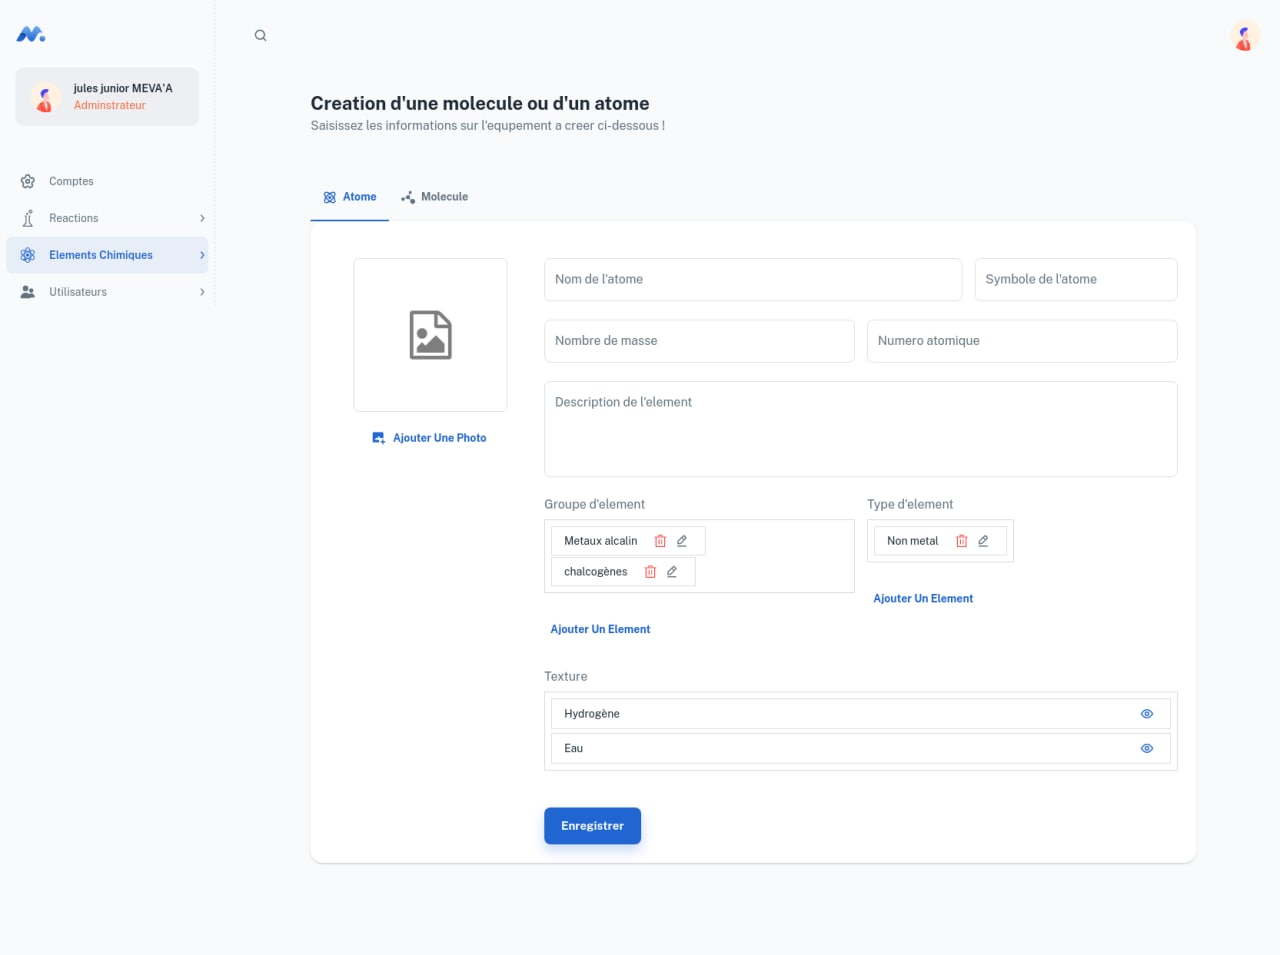
\includegraphics[width=1\textwidth]{img/iec}
	\caption{IHM formulaire de création des éléments chimiques}
	\label{fig:mesh1}
\end{figure}

Ce formulaire permet la création d'un élément chimique (Atome et molécule) et celà en fonction de notre role, seul l'administrateur à le droit de créer des atomes tandis que la création des molécules est autorisée à tous les utilisateurs.

\subsubsection{Code source backend}

\begin{figure}[H]
	\centering
	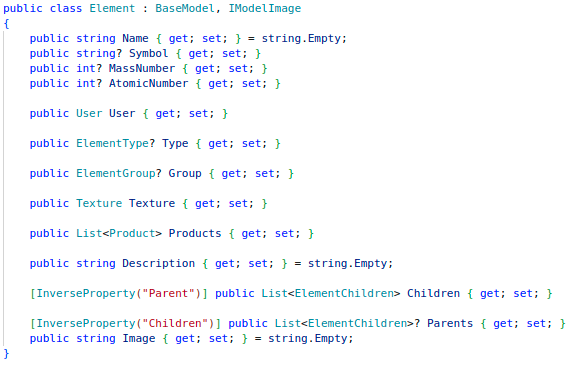
\includegraphics[width=1\textwidth]{img/met}
	\caption{Code backend du model d'élément chimique}
	\label{fig:mesh1}
\end{figure}

Il est question ici de la définition du model d'élément chimique qui sera stocké en base de données.

\begin{figure}[H]
	\centering
	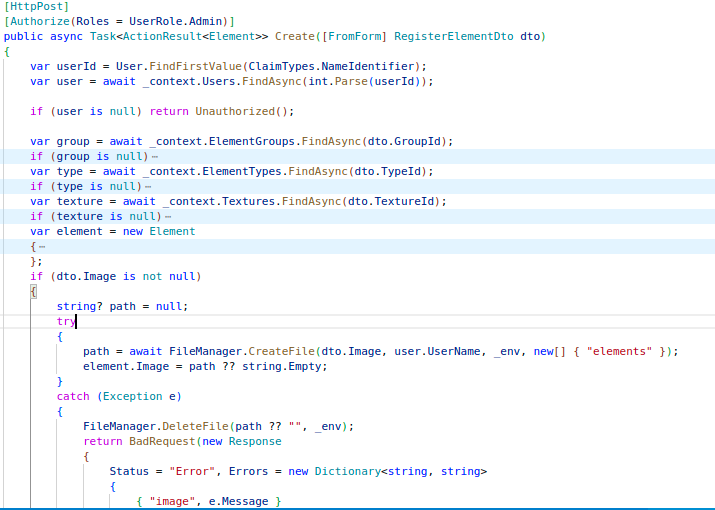
\includegraphics[width=1\textwidth]{img/cep}
	\caption{Code backend du cas d'utilisation de la création d'élément chimique}
	\label{fig:mesh1}
\end{figure}

Il est question ici du code permettant la création d'un élément chimique (atomes).

\begin{figure}[H]
	\centering
	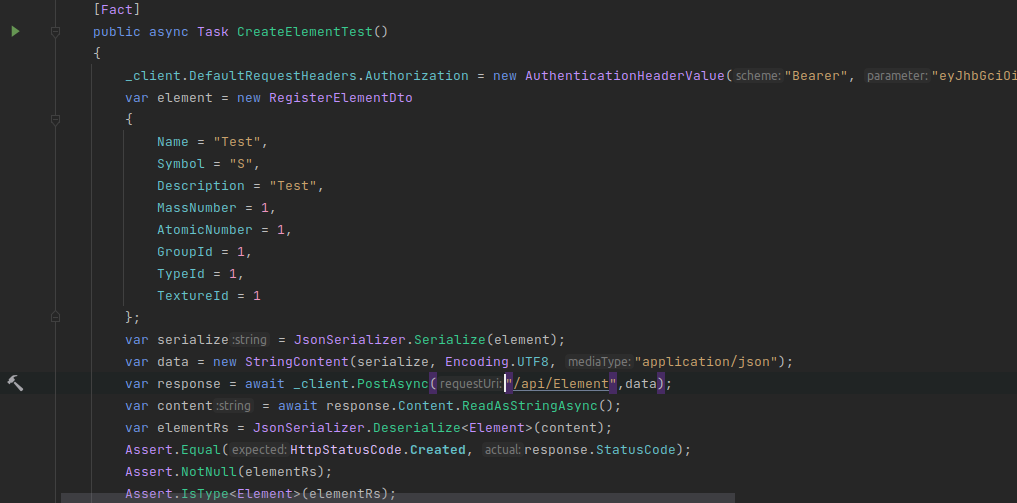
\includegraphics[width=1\textwidth]{img/cet}
	\caption{Code backend du test unitaire du cas d'utilisation de la création d'élément chimique}
	\label{fig:mesh1}
\end{figure}

Il est question ici d'une partie du code de test de la fonctionnalités de création d'élément chimique.

\begin{figure}[H]
	\centering
	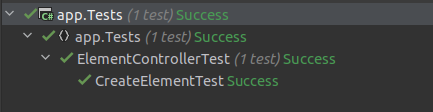
\includegraphics[width=1\textwidth]{img/ute}
	\caption{Résultat du test unitaire du cas d'utilisation de la création d'élément chimique}
	\label{fig:mesh1}
\end{figure}

Nous avons ici le resultat du test unitaire du cas d'utilisation de la création d'élément chimique, qui s'avère concluent.

\subsubsection{Code source frontend}

\begin{figure}[H]
	\centering
	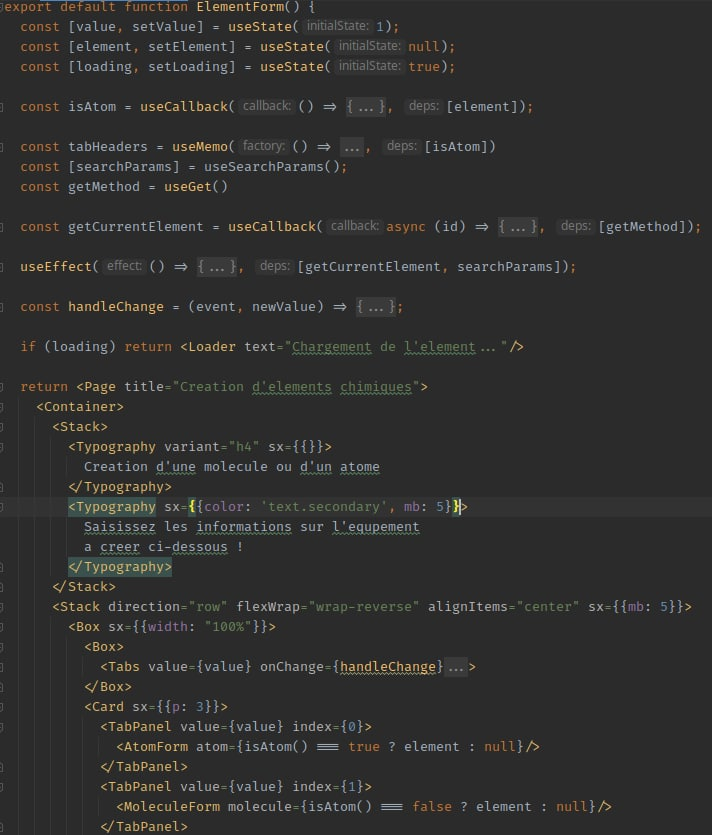
\includegraphics[width=1\textwidth]{img/fec}
	\caption{Code frontend du cas d'utilisation de la création d'élément chimique}
	\label{fig:mesh1}
\end{figure}

Il est question ici du code React permettant le rendu de la page de création d'élément chimique.

\subsection{Listing des éléments chimiques}

\subsubsection{Interface de listing des éléments chimiques}

\begin{figure}[H]
	\centering
	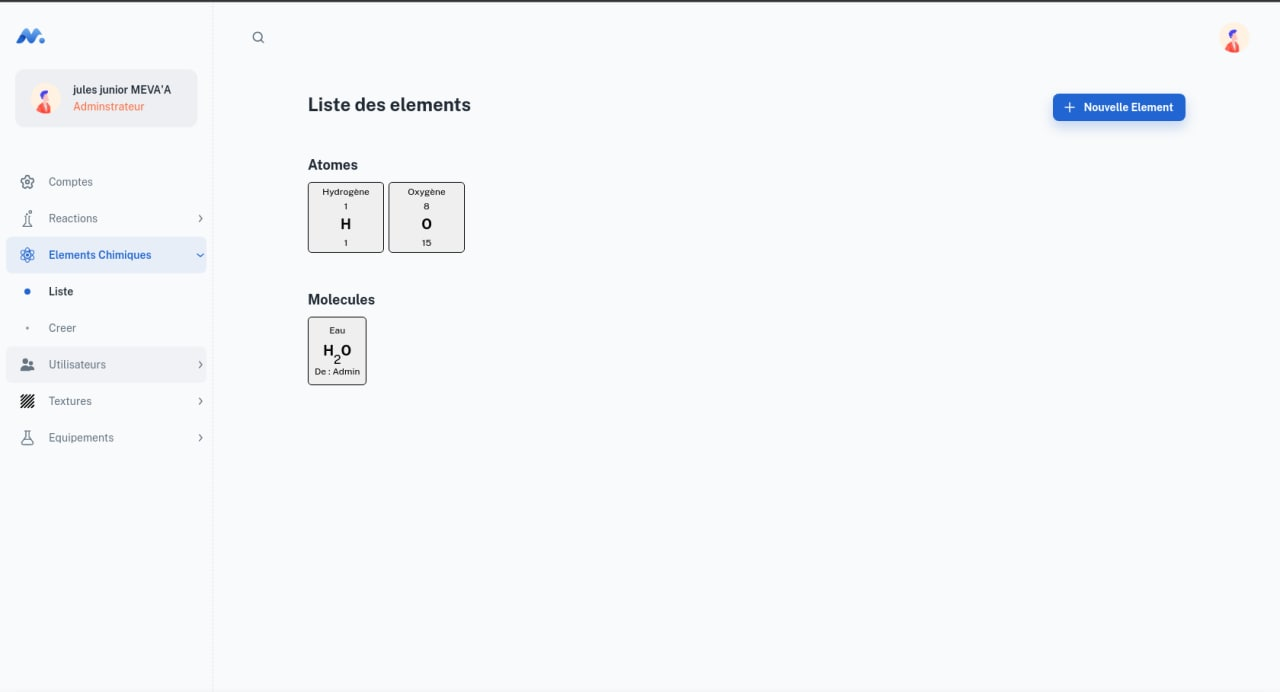
\includegraphics[width=1\textwidth]{img/ietl}
	\caption{IHM du listing des éléments chimiques}
	\label{fig:mesh1}
\end{figure}

Cette interface permet la listing des éléments chimiques (Atome et molécule) enregistrés dans la base de données.

\subsubsection{Code source backend}

\begin{figure}[H]
	\centering
	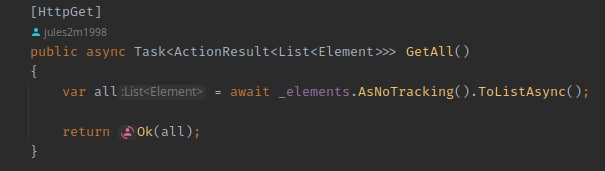
\includegraphics[width=1\textwidth]{img/cetl}
	\caption{Code backend du controller de listing des éléments chimiques}
\end{figure}

Il est question ici du code backend permettant la recupération des élements chimiques en base de données afin de les communiquer à l'interface pour un rendu à l'utilisateur (enseignants ou administrateurs).

\begin{figure}[H]
	\centering
	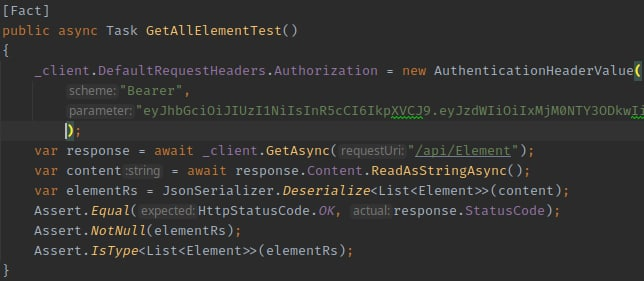
\includegraphics[width=1\textwidth]{img/utetlist2}
	\caption{Code backend du test unitaire du cas d'utilisation de la listing des éléments chimiques}
\end{figure}

Il est question ici du code de test unitaire de la fonctionnalités de listing des éléments chimiques.

\begin{figure}[H]
	\centering
	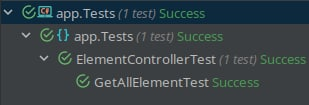
\includegraphics[width=1\textwidth]{img/utetlist}
	\caption{Resultat du test unitaire de la fonctionnalités de listing des éléments chimiques}
\end{figure}

Nous avons ici le resultat du test unitaire de la fonctionnalités de listing des éléments chimiques, qui s'avère concluent.

\subsubsection{Code source frontend}

\begin{figure}[H]
	\centering
	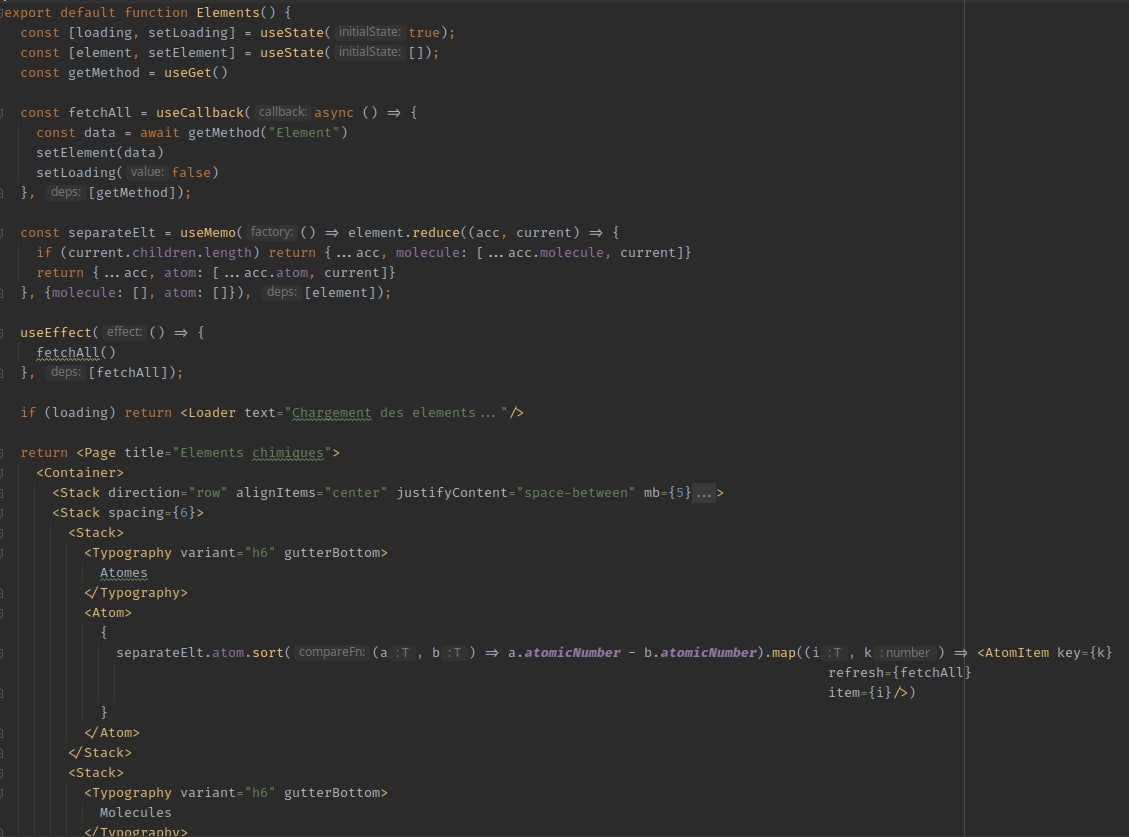
\includegraphics[width=1\textwidth]{img/fetl}
	\caption{Code frontend du cas d'utilisation de la listing des éléments chimiques}
\end{figure}

Il est question ici du code React permettant le rendu de la page de listing des éléments chimiques.

\subsection{Création des réactions chimiques}

\subsubsection{Interface du formulaire de création des réactions chimiques}

\begin{figure}[H]
	\centering
	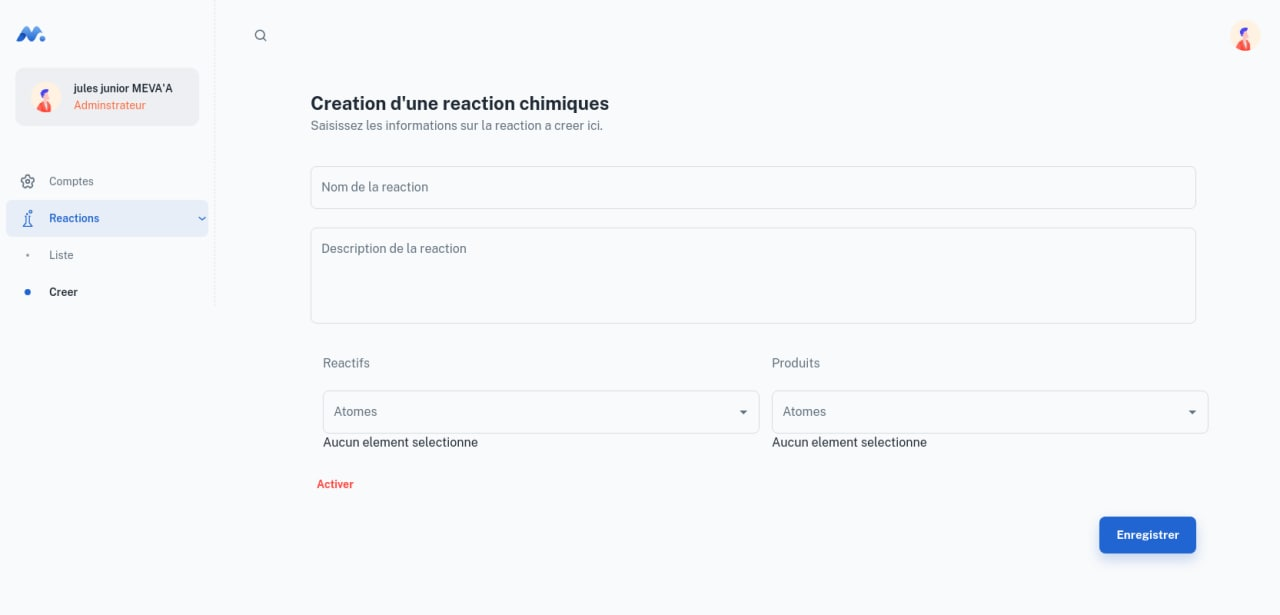
\includegraphics[width=1\textwidth]{img/icrc}
	\caption{IHM formulaire de création des réactions chimiques}
\end{figure}

Ce formulaire permet la création d'une réaction chimique à un utilisateur. Il est question ici de lui donner un nom, un description,
lister les réactifs et les produits de la réaction et de l'activer ou la désactiver.

\subsubsection{Code source backend}

\begin{figure}[H]
	\centering
	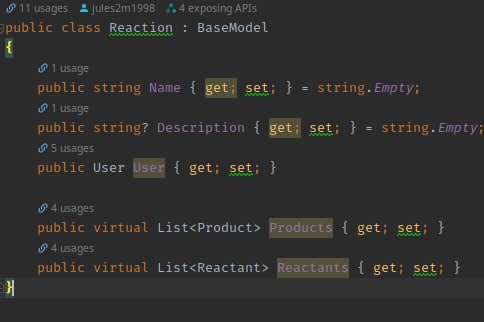
\includegraphics[width=1\textwidth]{img/mre}
	\caption{Code backend du model de réaction}
\end{figure}

Il est question ici de la représentation du modèle d'une réaction chimique qui sera stocké en base de données.

\begin{figure}[H]
	\centering
	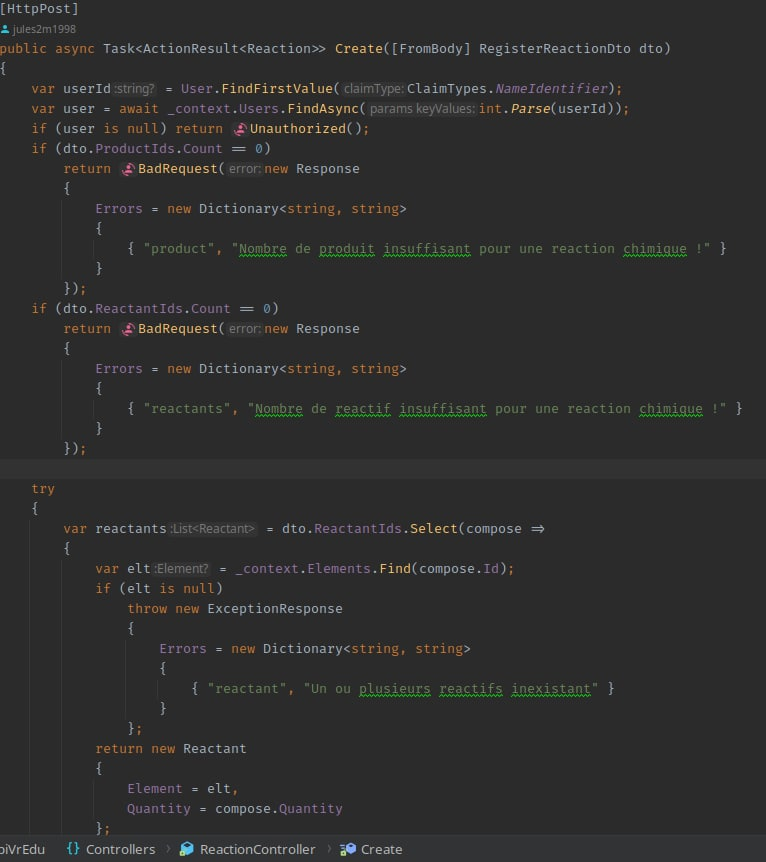
\includegraphics[width=1\textwidth]{img/crec}
	\caption{Code backend du controller de création des réactions chimiques}
\end{figure}

Il est question ici du code permettant la sauvegarde en base de données d'une réaction chimique, cette action n'est possible qu'une fois authentifié.

\begin{figure}[H]
	\centering
	\includegraphics[width=1\textwidth]{img/creac}
	\caption{Code backend du test unitaire du cas d'utilisation de la création d'une réaction chimique}
\end{figure}

Il est question ici d'une partie du code de test de la fonctionnalités de création d'une réaction chimique.

\begin{figure}[H]
	\centering
	\includegraphics[width=1\textwidth]{img/utcre}
	\caption{Resultat du test unitaire de la fonctionnalités de création d'une réaction chimique}
\end{figure}

Nous avons ici le resultat du test unitaire de la fonctionnalités de création d'une réaction chimique, qui s'avère concluent.

\subsubsection{Code source frontend}

\begin{figure}[H]
	\centering
	\includegraphics[width=1\textwidth]{img/frec}
	\caption{Code frontend du cas d'utilisation de la création d'une réaction chimique}
\end{figure}

Il est question ici du code React permettant le rendu de la page de création d'une réaction chimique.

\subsection{Listing des réactions chimiques}

\subsubsection{Interface de listing des réactions chimiques}

\begin{figure}[H]
	\centering
	\includegraphics[width=1\textwidth]{img/ilrc}
	\caption{IHM du listing des réactions chimiques}
\end{figure}

Cette interface permet de lister les réactions d'un utilisateur connecté.

\subsubsection{Code source backend}

\begin{figure}[H]
	\centering
	\includegraphics[width=1\textwidth]{img/clrea}
	\caption{Code backend du controller de listing des réactions chimiques}
\end{figure}

Il est question ici du code backend permettant la recupération en base de données des réactions chimiques créé par l'utilisateur connecté afin de les communiquer à l'interface pour un rendu.

\begin{figure}[H]
	\centering
	\includegraphics[width=1\textwidth]{img/utreaall}
	\caption{Code backend du test unitaire du cas d'utilisation de la listing des réactions chimiques}
\end{figure}

Il est question ici du code de test unitaire de la fonctionnalités de listing des réactions chimiques.

\begin{figure}[H]
	\centering
	\includegraphics[width=1\textwidth]{img/utrcr}
	\caption{Resultat du test unitaire de la fonctionnalités de listing des réactions chimiques}
\end{figure}

Nous avons ici le resultat du test unitaire de la fonctionnalités de listing des réactions chimiques, qui s'avère concluent.

\subsubsection{Code source frontend}

\begin{figure}[H]
	\centering
	\includegraphics[width=1\textwidth]{img/frl}
	\caption{Code frontend du cas d'utilisation de la listing des réactions chimiques}
\end{figure}

Il est question ici du code React permettant le rendu de la page de listing des réactions chimiques.
\chapter*{Conclusion}

Il était question pour nous de concevoir un environnement virtuelle permettant la simulation d'un laboratoire de chimie, afin de permettre aux apprenants d'évoluer dans un environnement sécurisé et moins onéreux qu'un laboratoire conventionnel.
Et pour ce faire nous avons d'une part fait un état de l'art afin de nous interesser aux travaux réalisés sur le sujet, d'autre part, grace à cet existant, nous avons éffectué une étude détaillée dans laquelle nous avons analysé la solution grâce à un cadrage de pragmatique et synthétique du projet, une identification du besoin et la conception du système grâce à des diagramme UML. 
Enfin, nous avons fait l'implémentation de la solution qui est passée par le choix des technologies utilisées à savoir Unreal Engine 5 pour la 3D, React \& React Dom pour le web, ASP.NET core web api pour le backend, PostgreSQL comme système de gestion des bases de données.

Le resultat obtenu est satisfaisant et nous estimons le taux de réalisation à environ 75\%. 
Notre solution n'étant pas une fin en soi, il serait judicieux de mettre sur pied la création de réactions types suivant le programme de chaque classe afin que les apprenants effectuent des réactions en fonction de leur programme sans que l'enseignant n'ait à intervenir.

% \LaTeX{} \cite{li20203d}

\nocite{*}
\bibliographystyle{plain} % We choose the "plain" reference style
\bibliography{refs} % Entries are in the refs.bib file
\clearpage
\setcounter{tocdepth}{3}
\tableofcontents % Table des matières
\end{document}